\chapter{Frequency Response Plots}
\label{ap:frfPlots}

%%%%%%%%%%%%%%%%%%%%%%%%%%%%%%%%%%%%%%%%%%%%%%%%%%%%%%%%%%%%%%%%%%%
\section{Ground Vibration Testing} %%%%%%%%%%%%%%%%%%%%%%%%%%%%%%%%
%%%%%%%%%%%%%%%%%%%%%%%%%%%%%%%%%%%%%%%%%%%%%%%%%%%%%%%%%%%%%%%%%%%

The plots each indicate the acceleration response at a location to an impulse input at a location. The locations are labeled by node number and direction. The locations of the respective nodes can be found in Figure \ref{fig:accelPlacement}.

\begin{figure}[H]
    \centering
    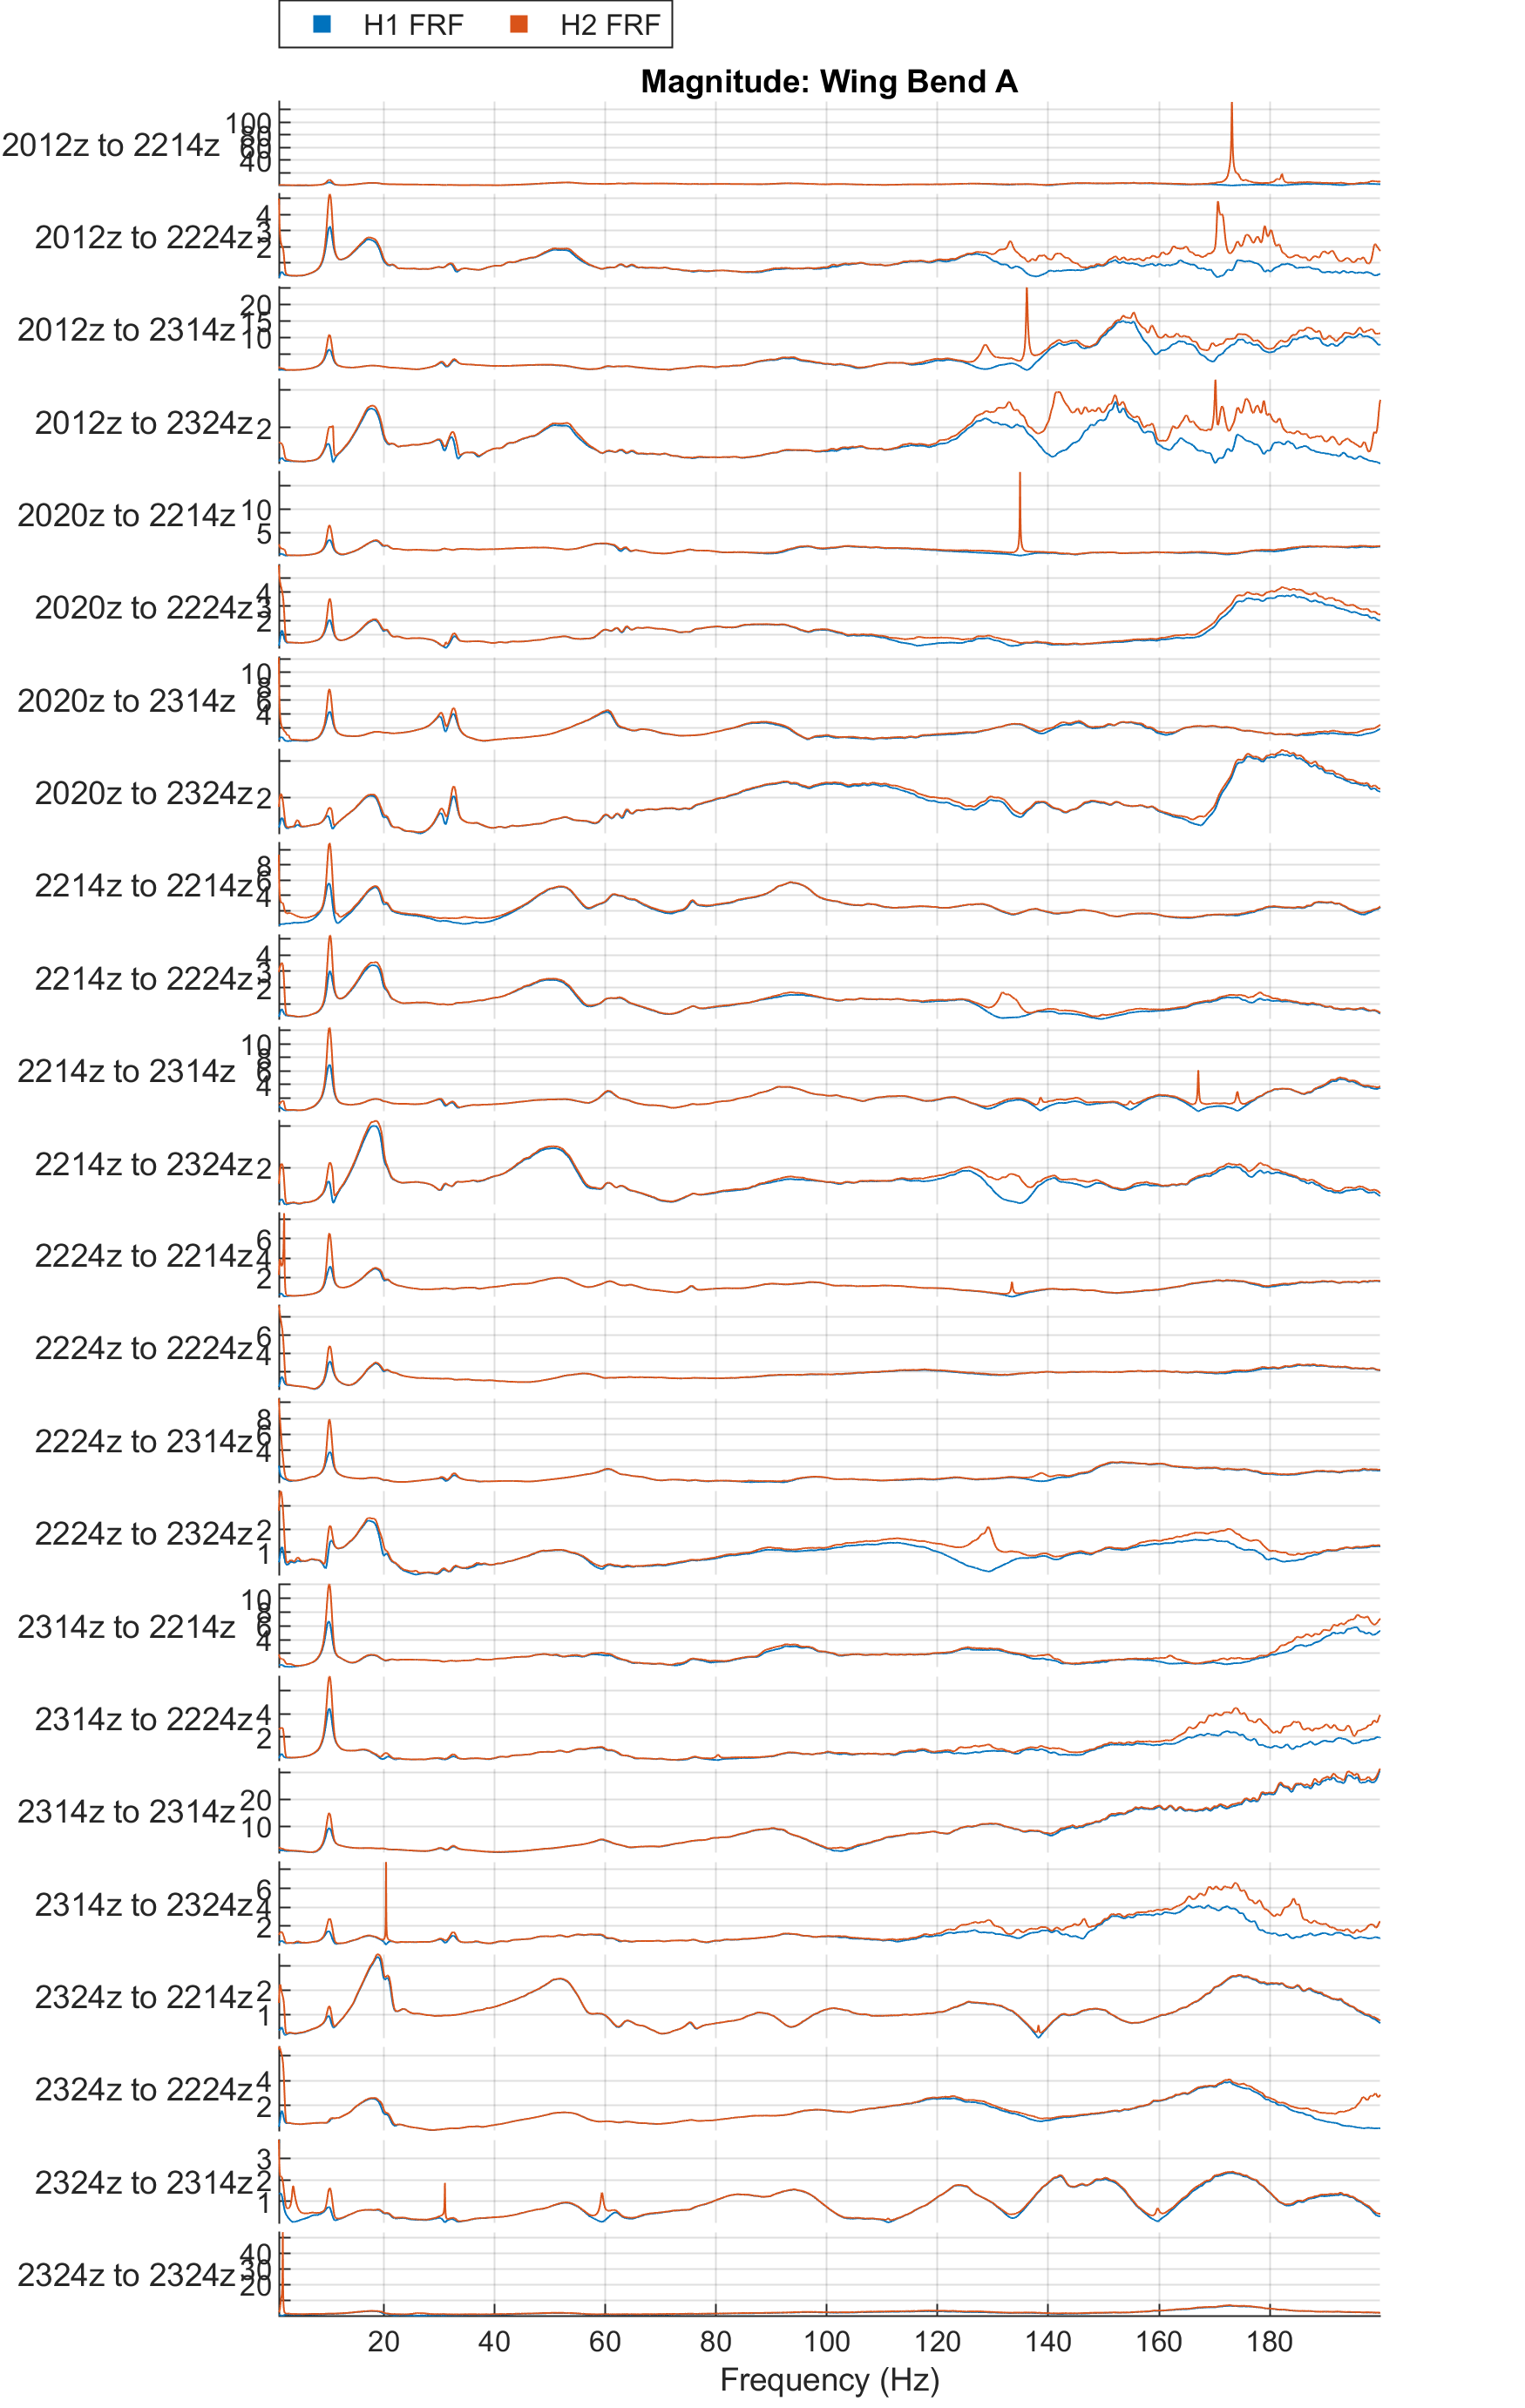
\includegraphics{figs/GVT/mag_Wing Bend A.png}
    \label{fig:mag_wingBendA}
\end{figure}
\begin{figure}[H]
    \centering
    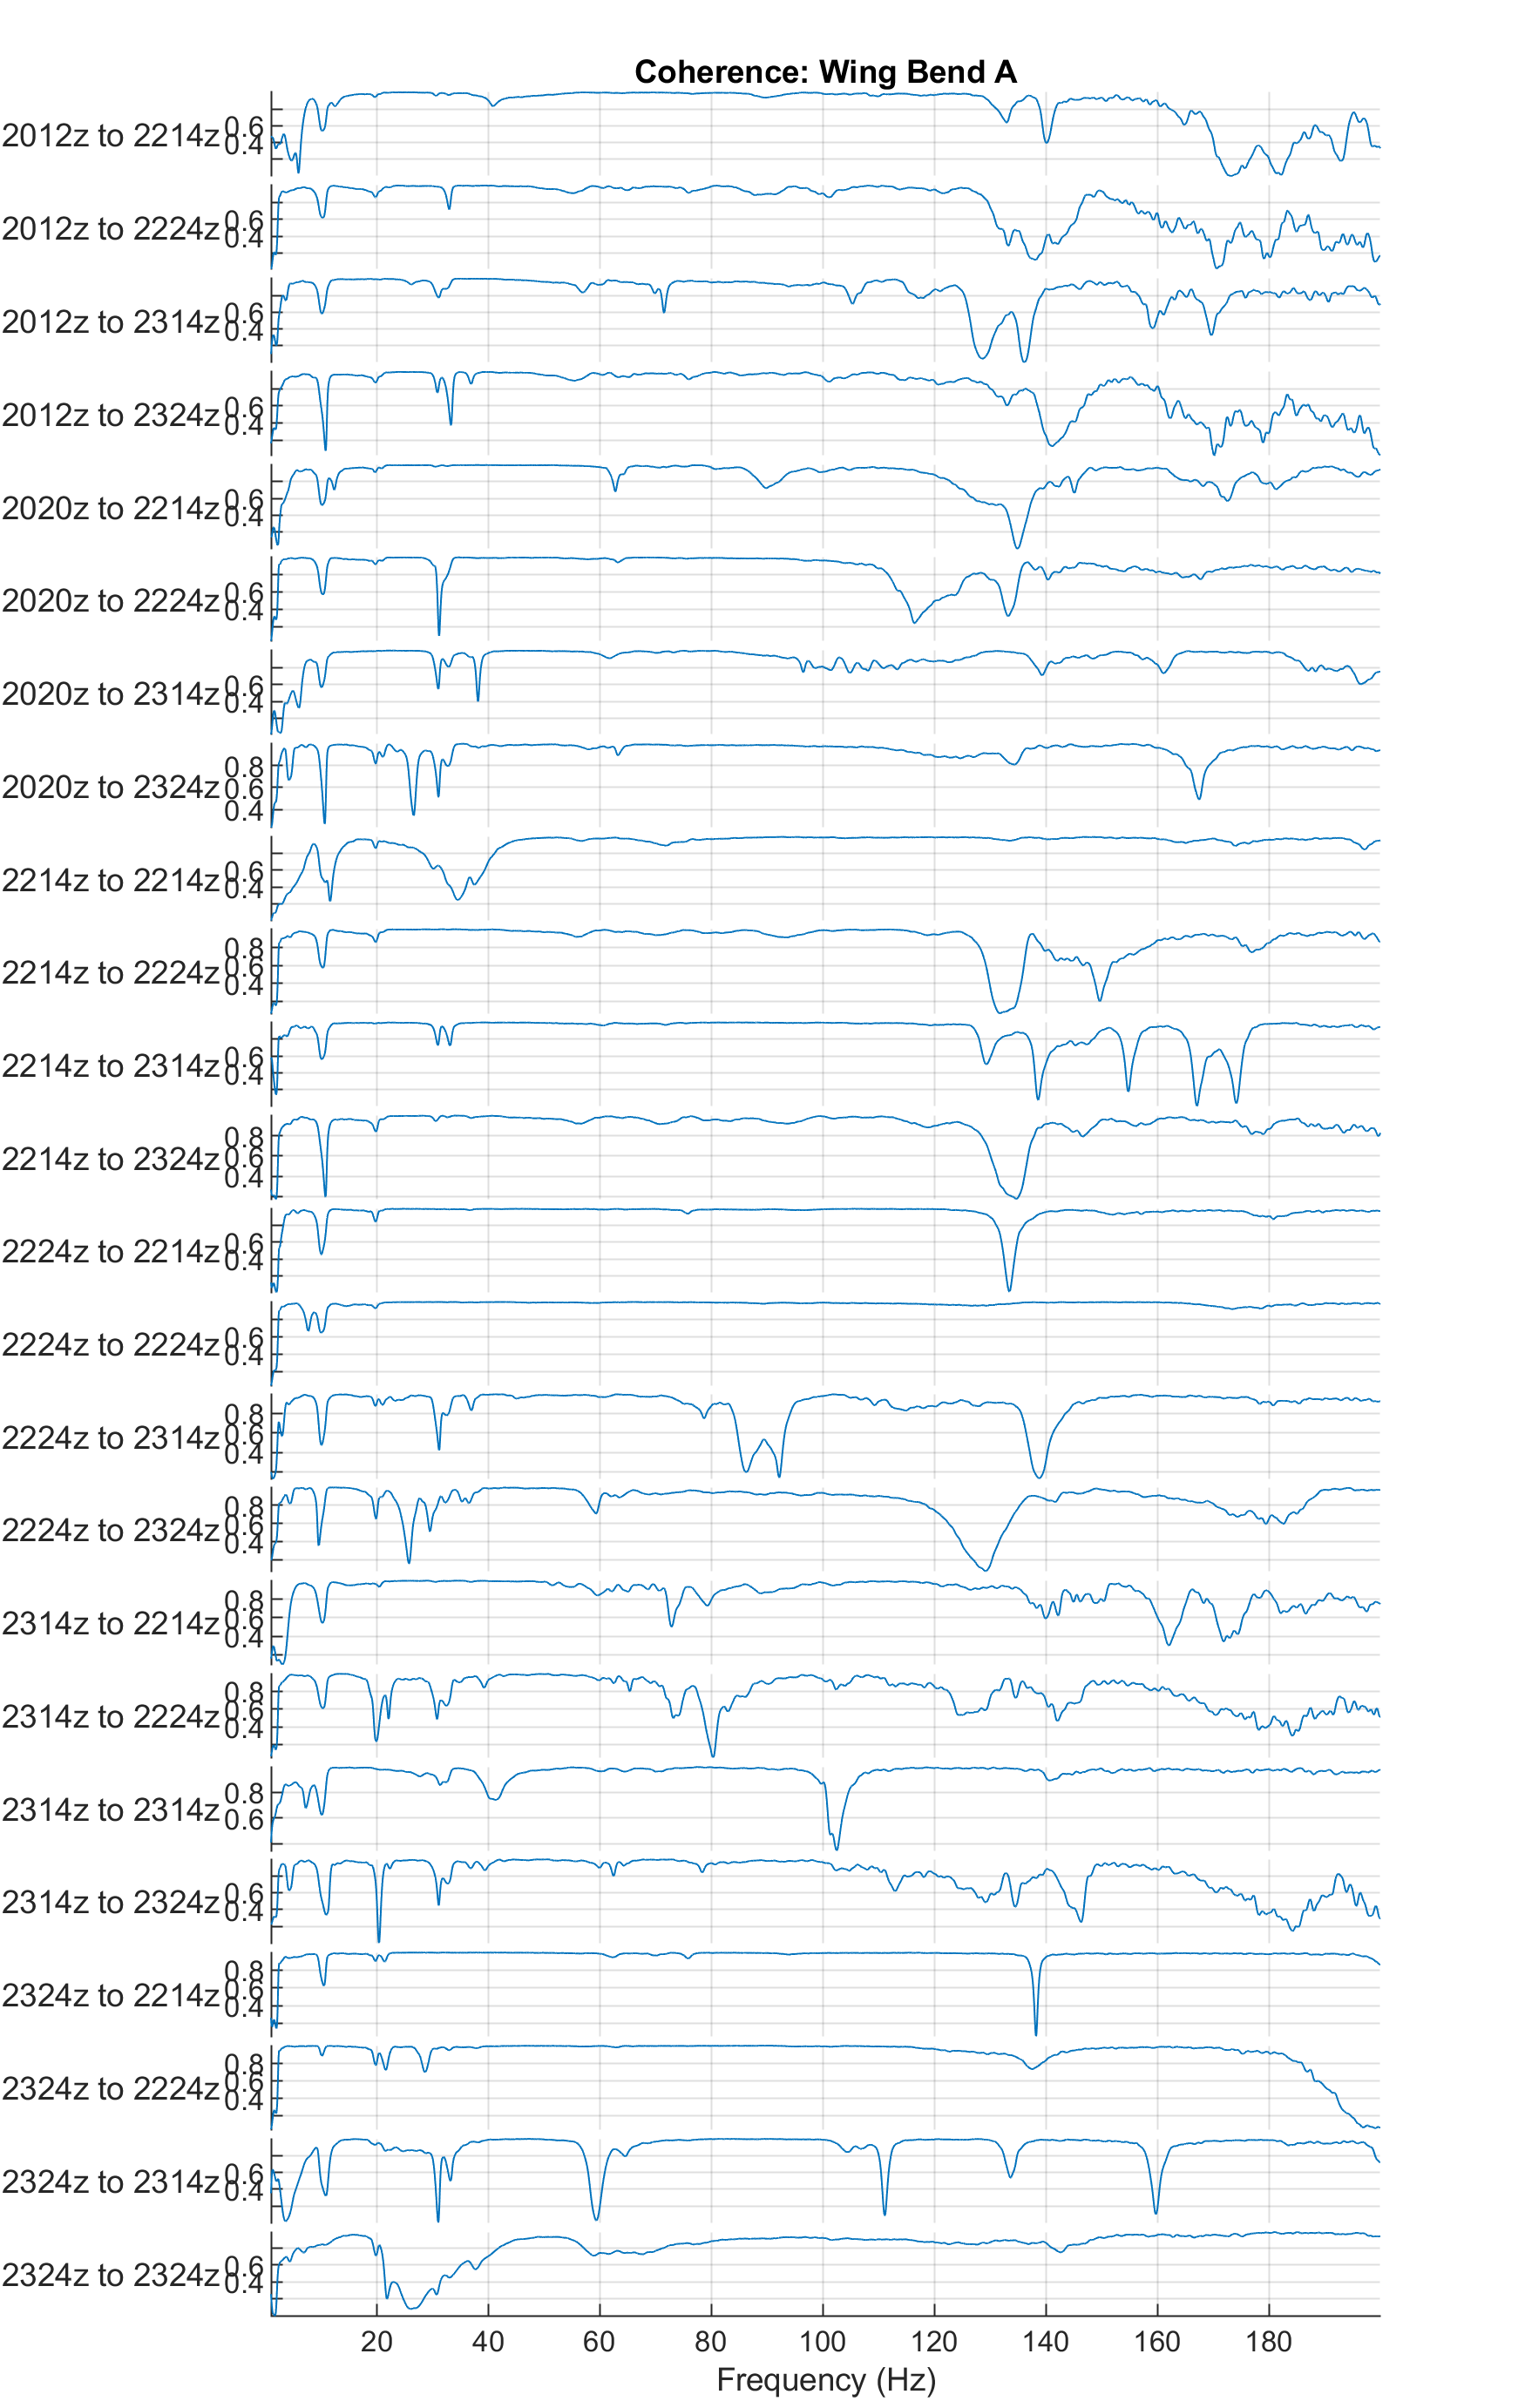
\includegraphics{figs/GVT/coh_Wing Bend A.png}
    \label{fig:coh_wingBendA}
\end{figure}

\begin{figure}[H]
    \centering
    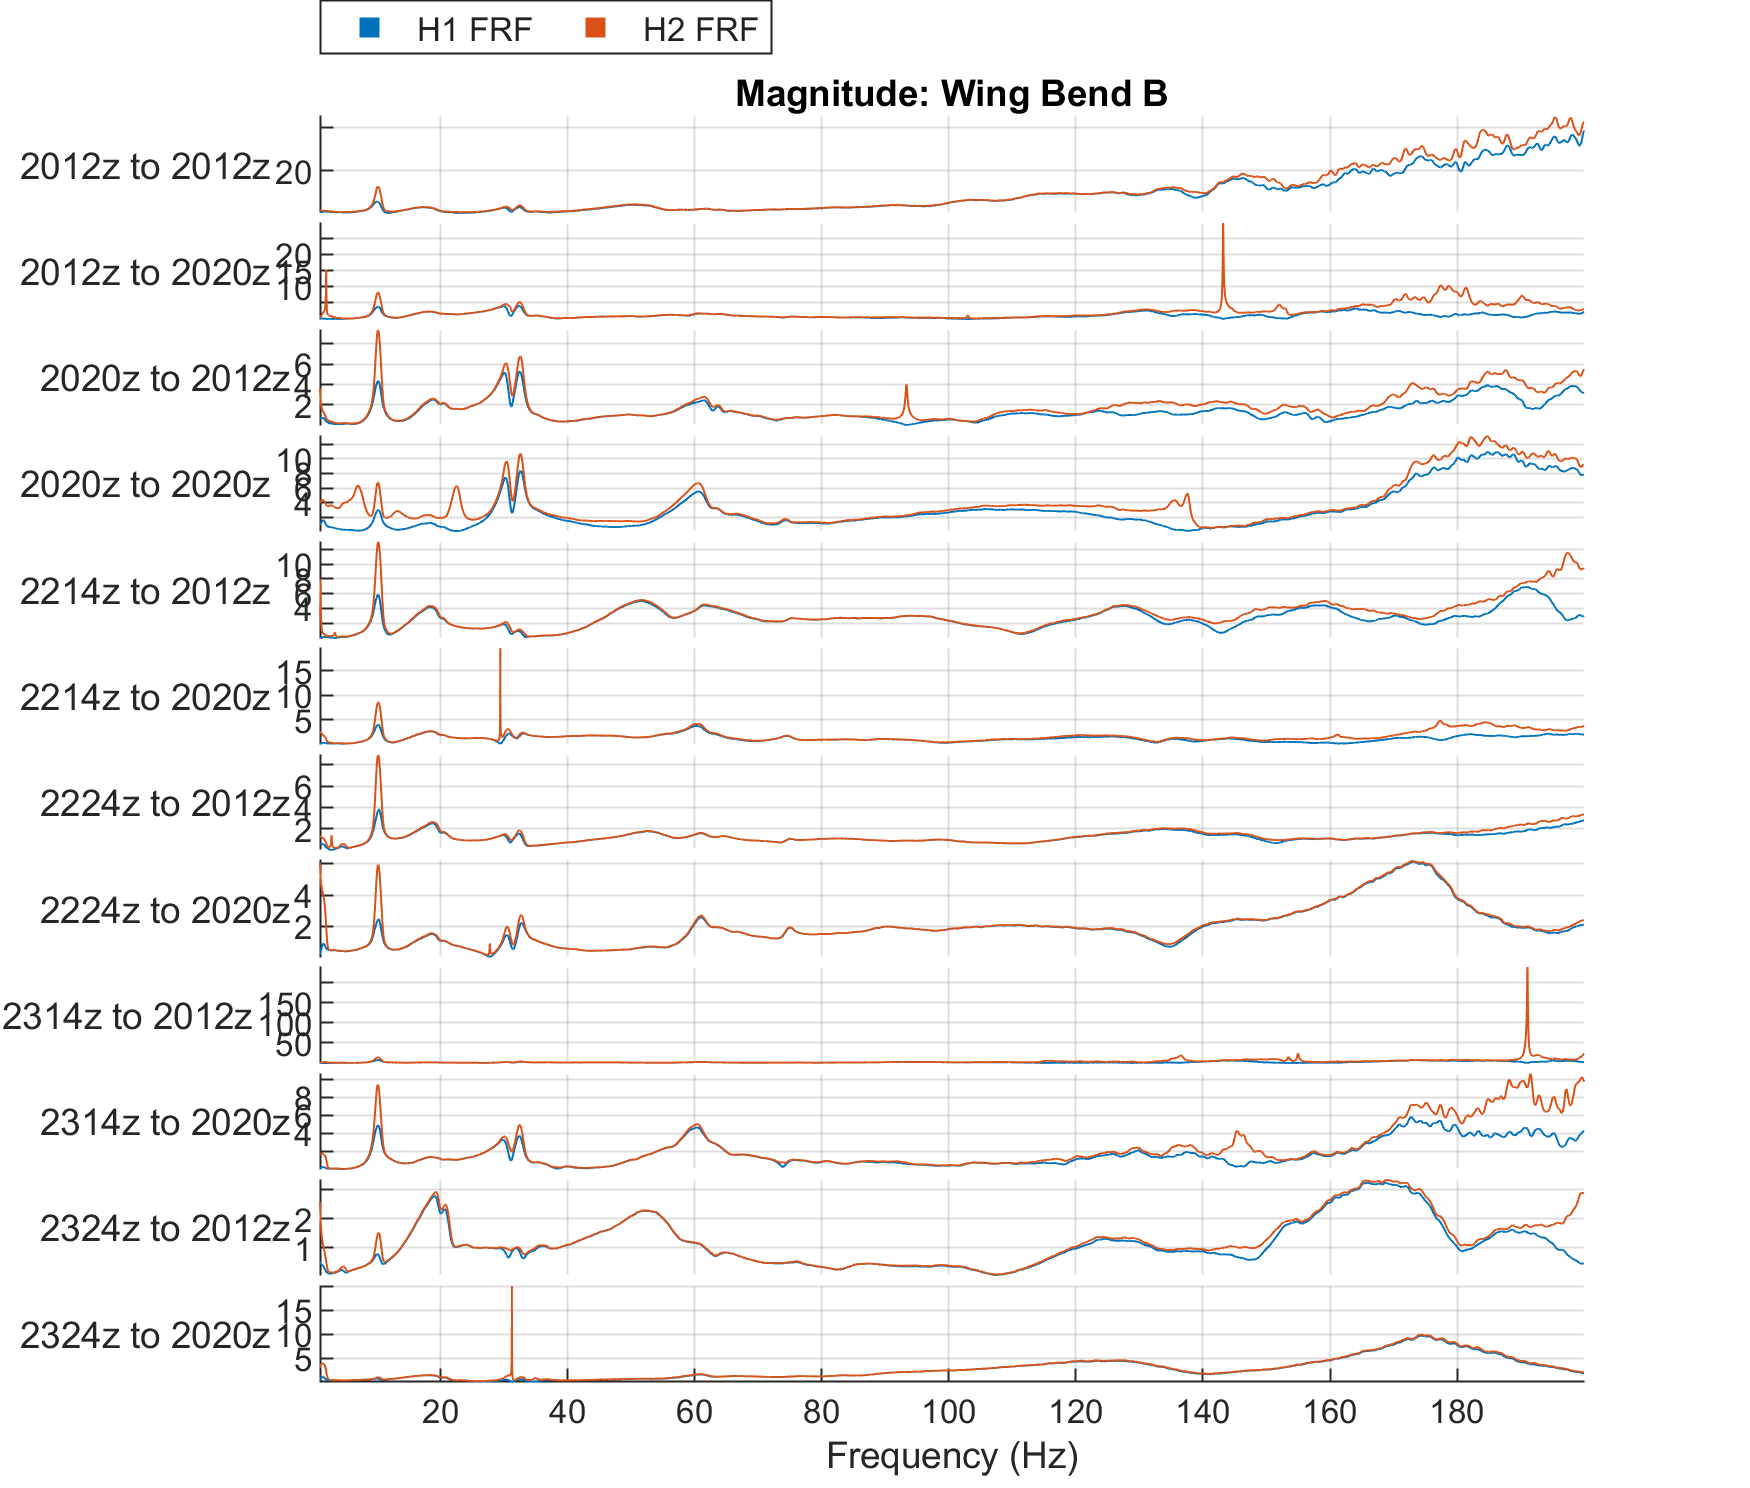
\includegraphics{figs/GVT/mag_Wing Bend B.png}
    \label{fig:mag_wingBendB}
\end{figure}
\begin{figure}[H]
    \centering
    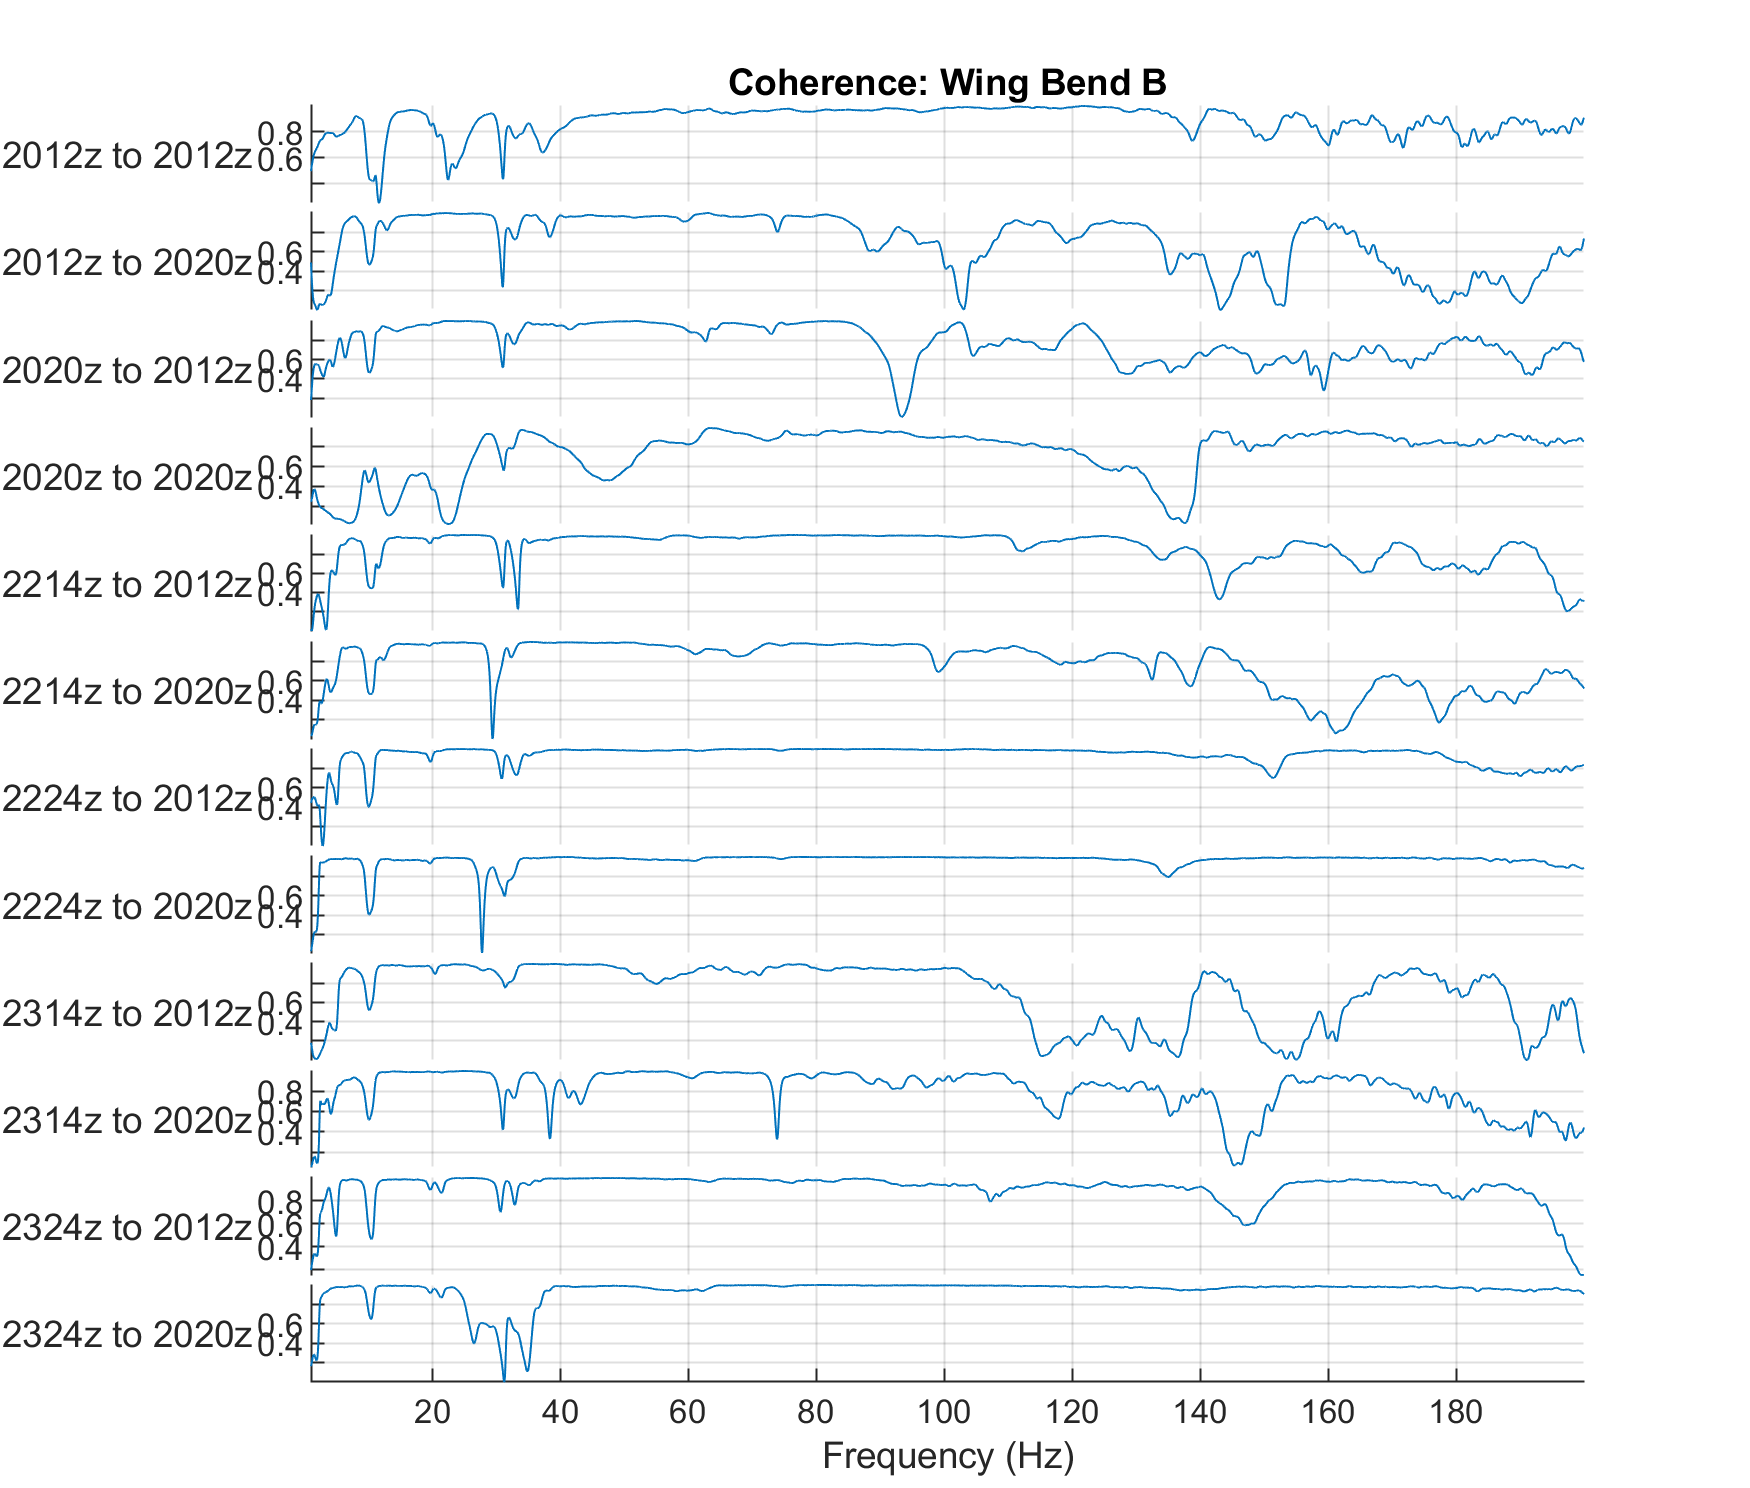
\includegraphics{figs/GVT/coh_Wing Bend B.png}
    \label{fig:coh_wingBendB}
\end{figure}

\begin{figure}[H]
    \centering
    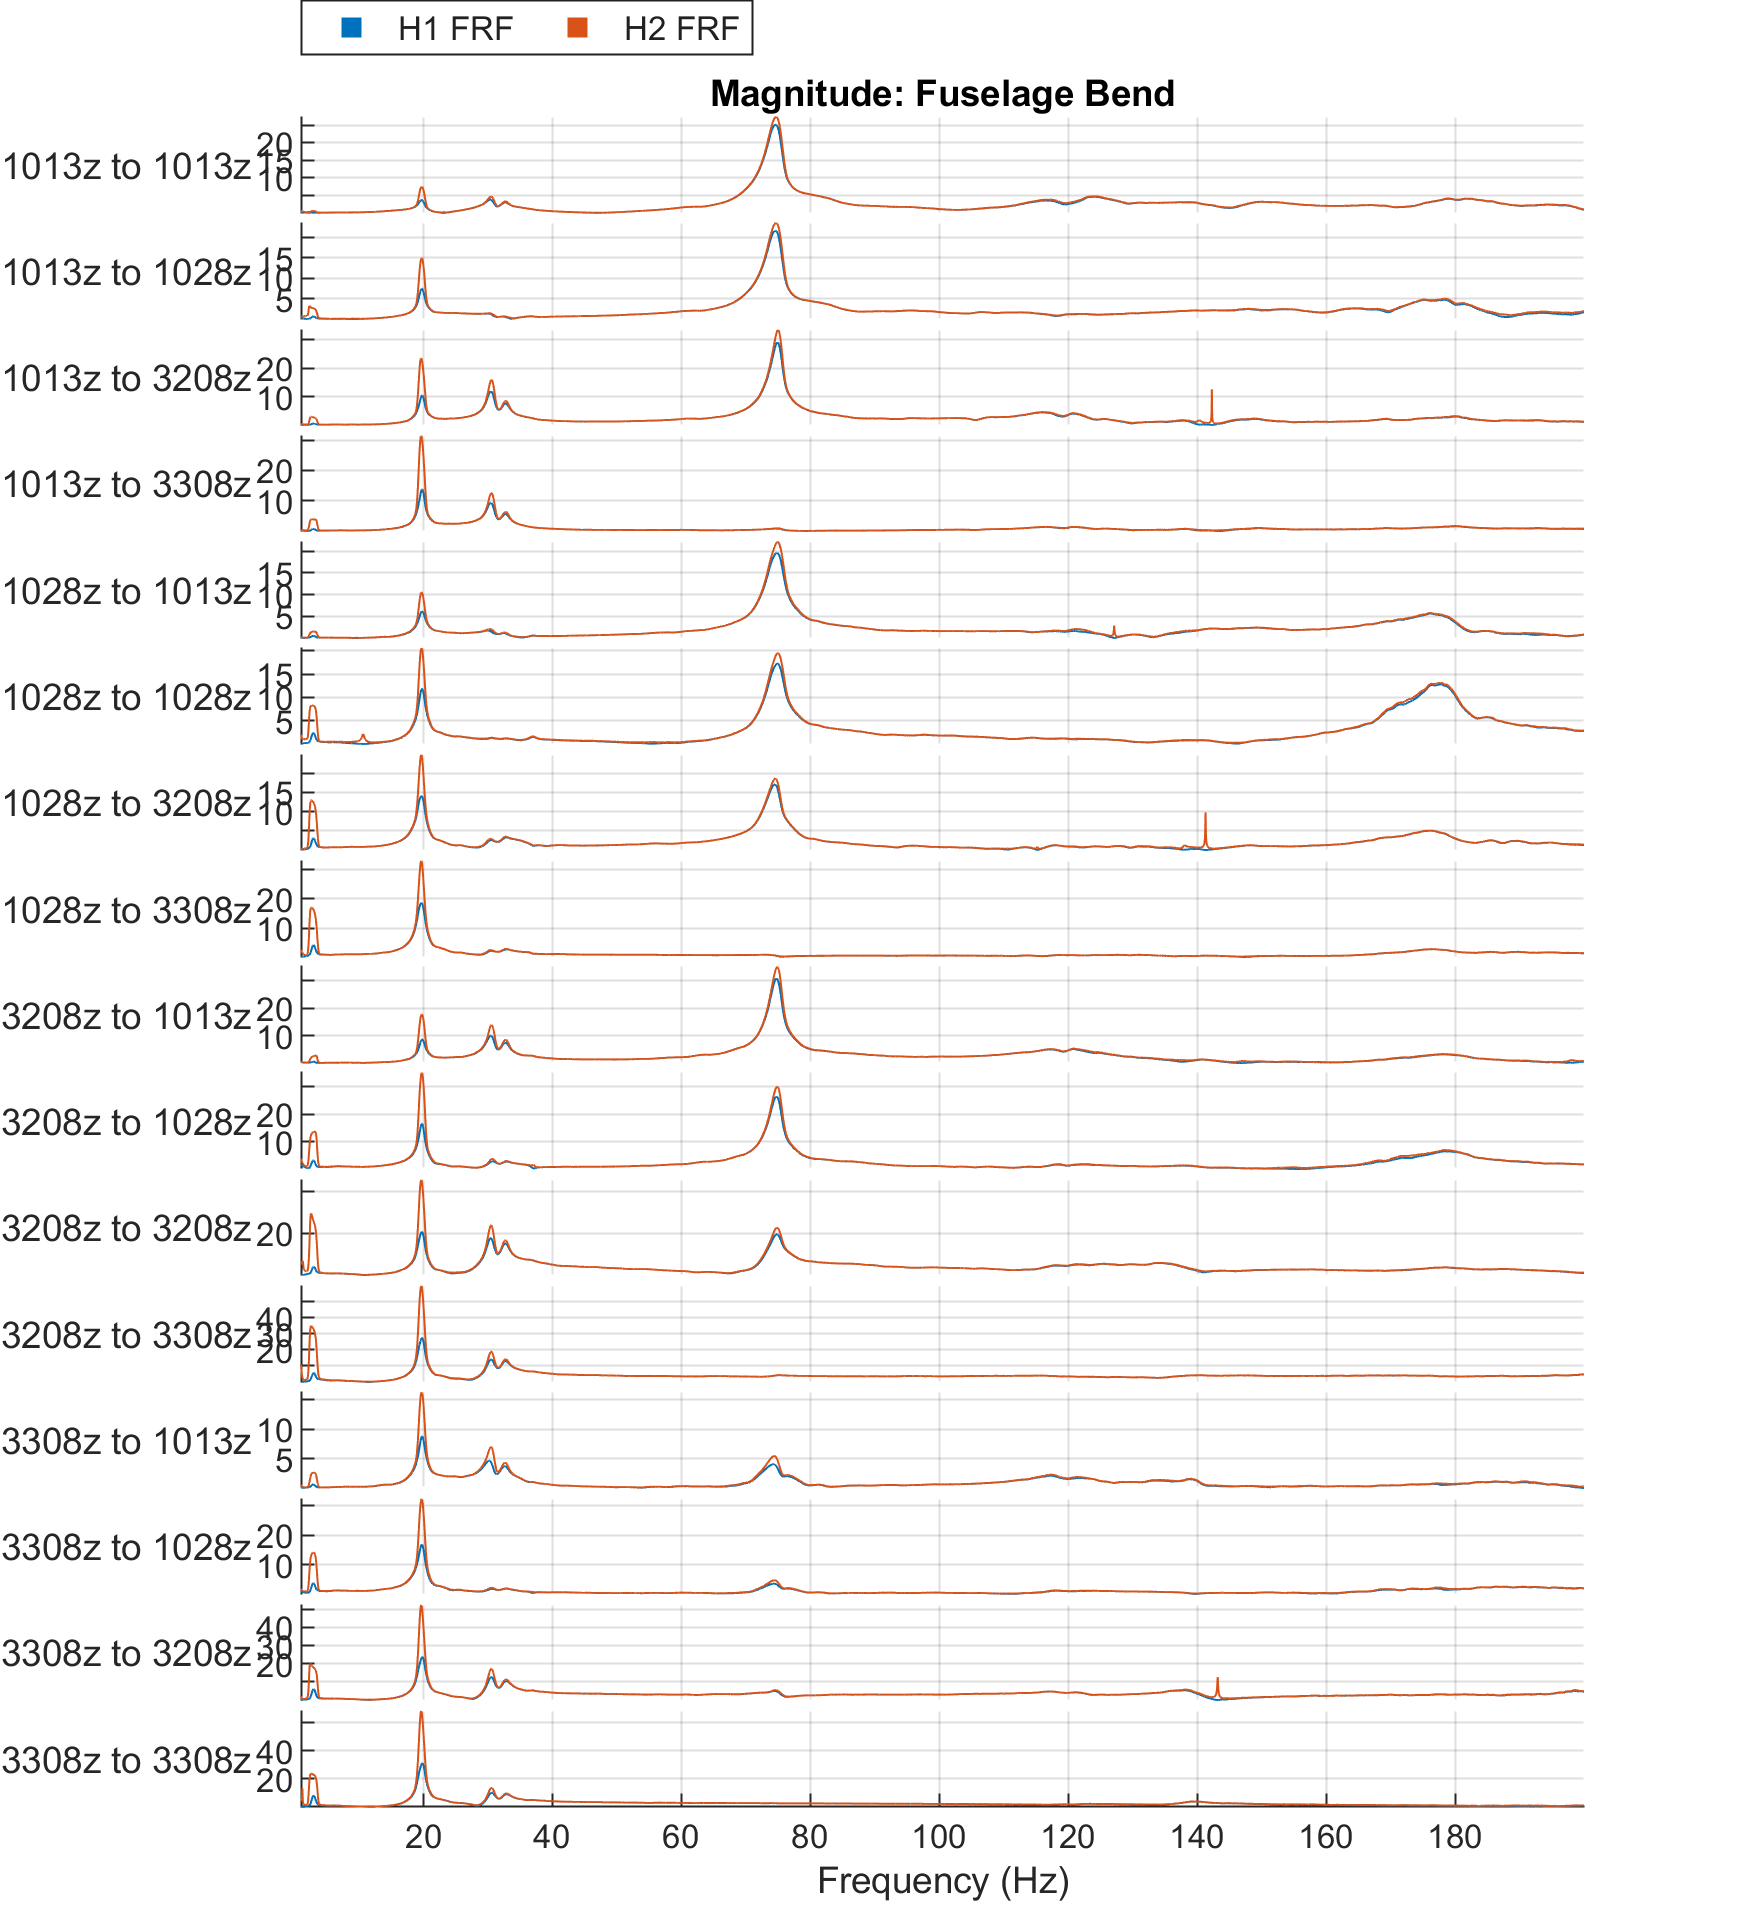
\includegraphics{figs/GVT/mag_Fuselage Bend.png}
    \label{fig:mag_fuseBend}
\end{figure}
\begin{figure}[H]
    \centering
    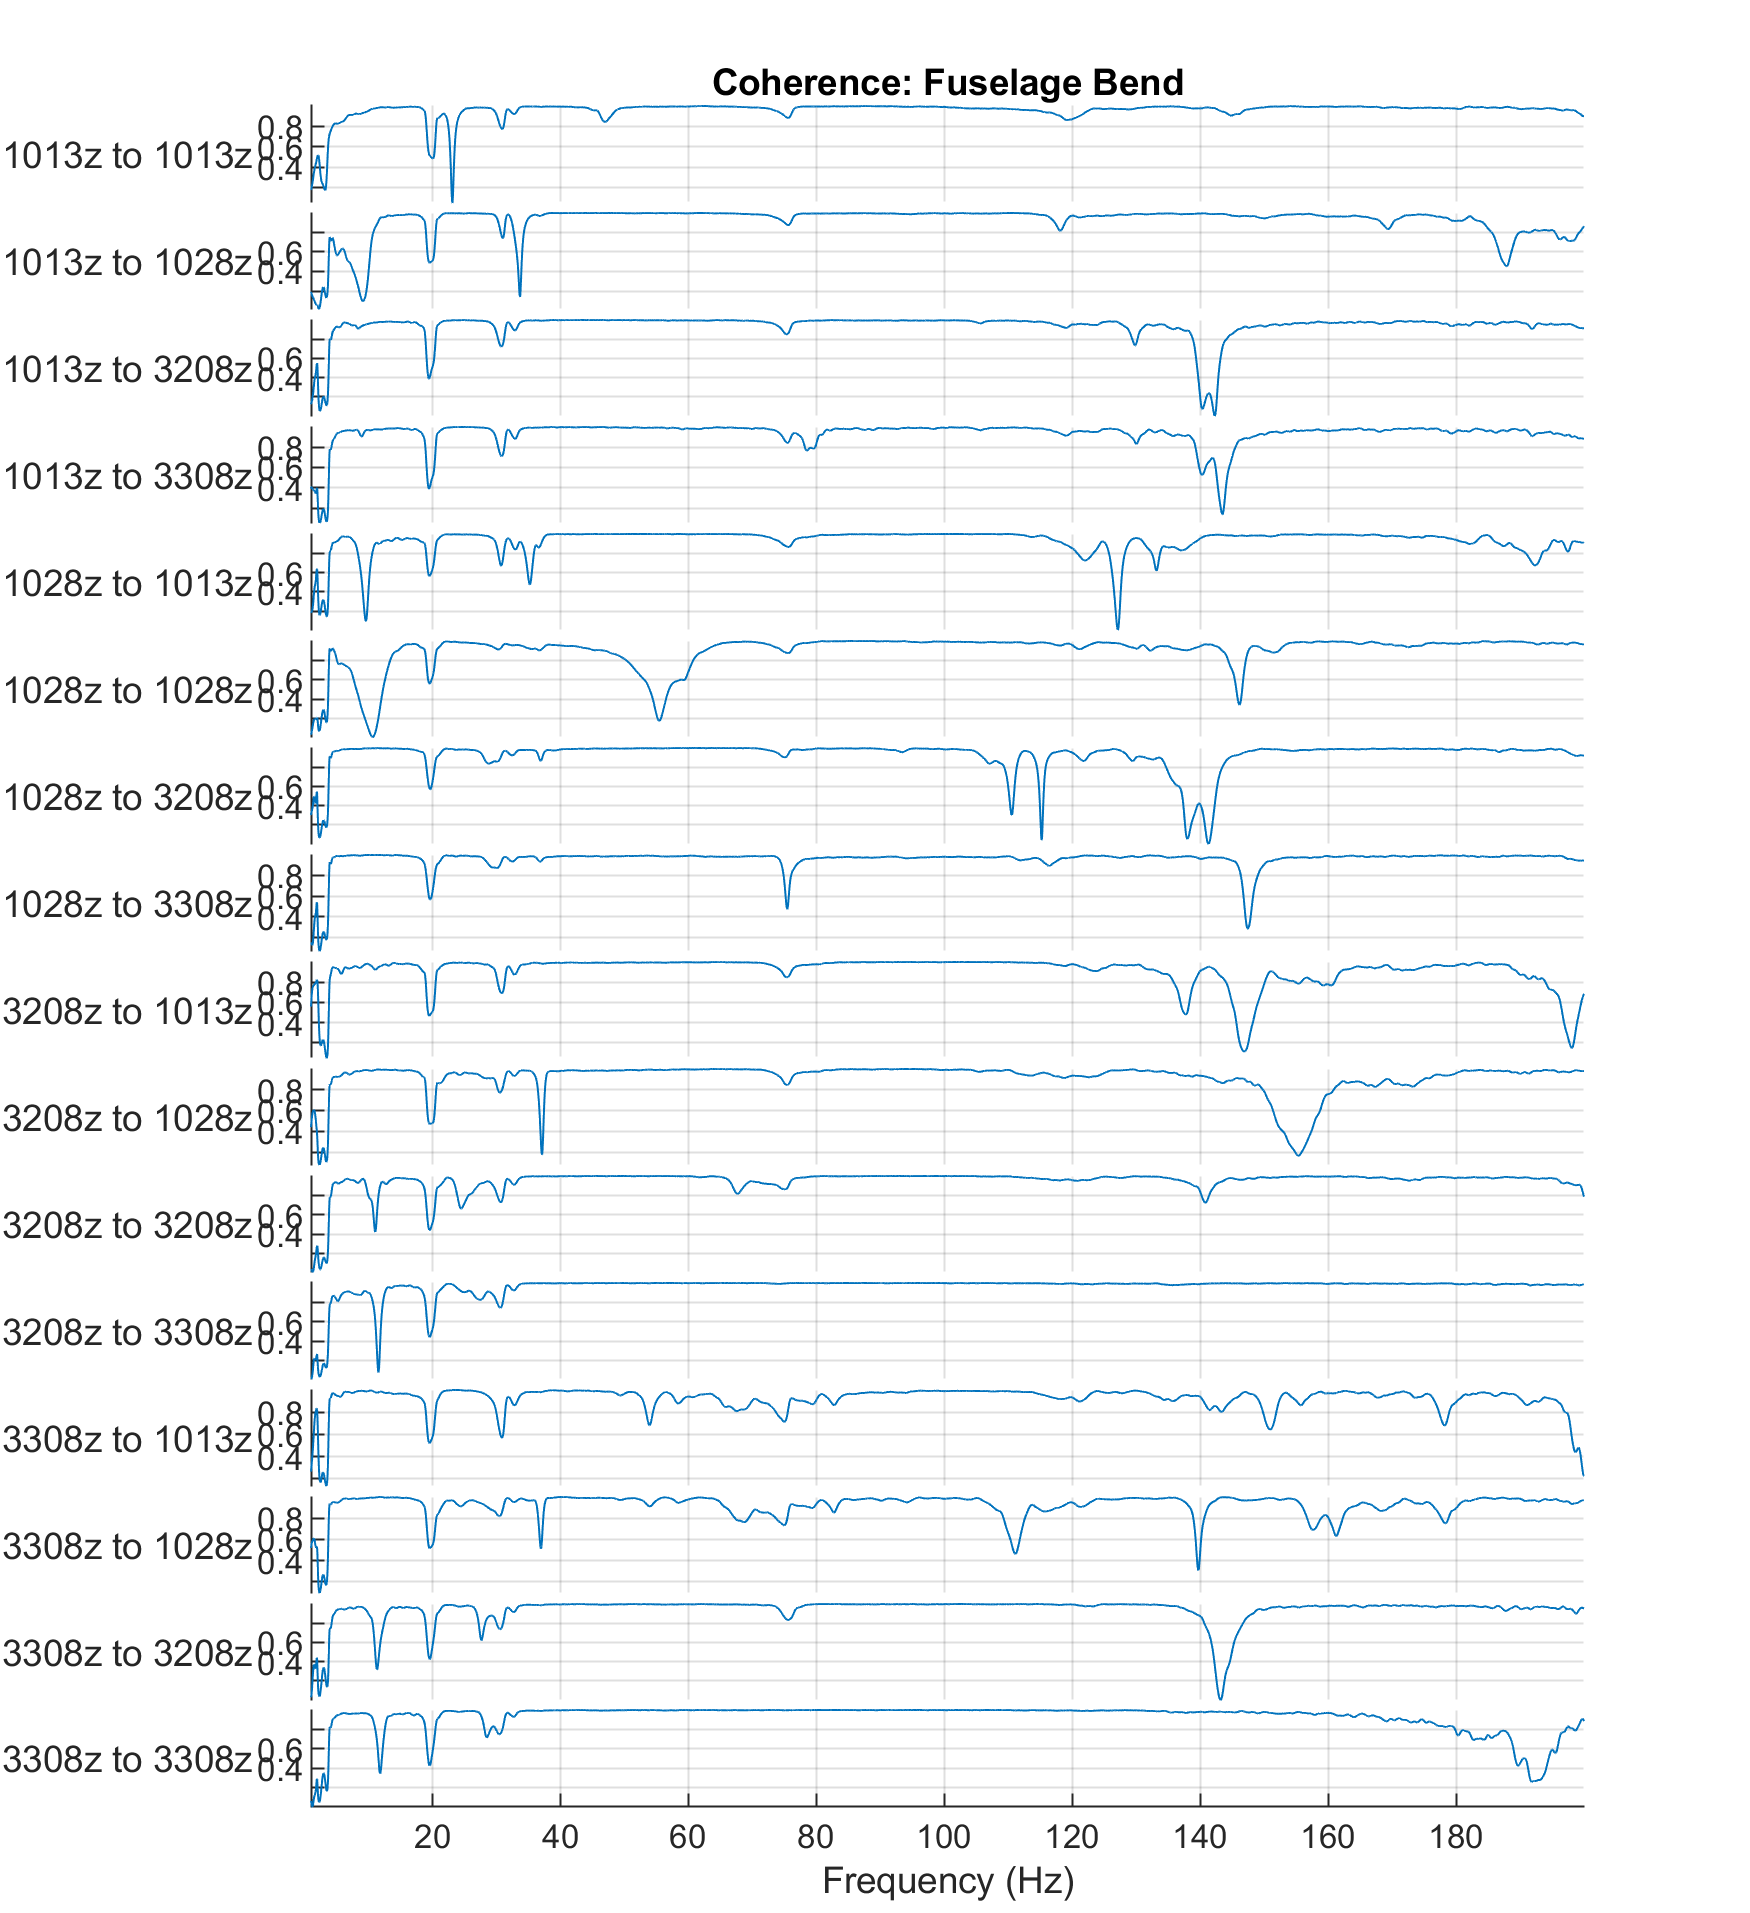
\includegraphics{figs/GVT/coh_Fuselage Bend.png}
    \label{fig:coh_fuseBend}
\end{figure}

\begin{figure}[H]
    \centering
    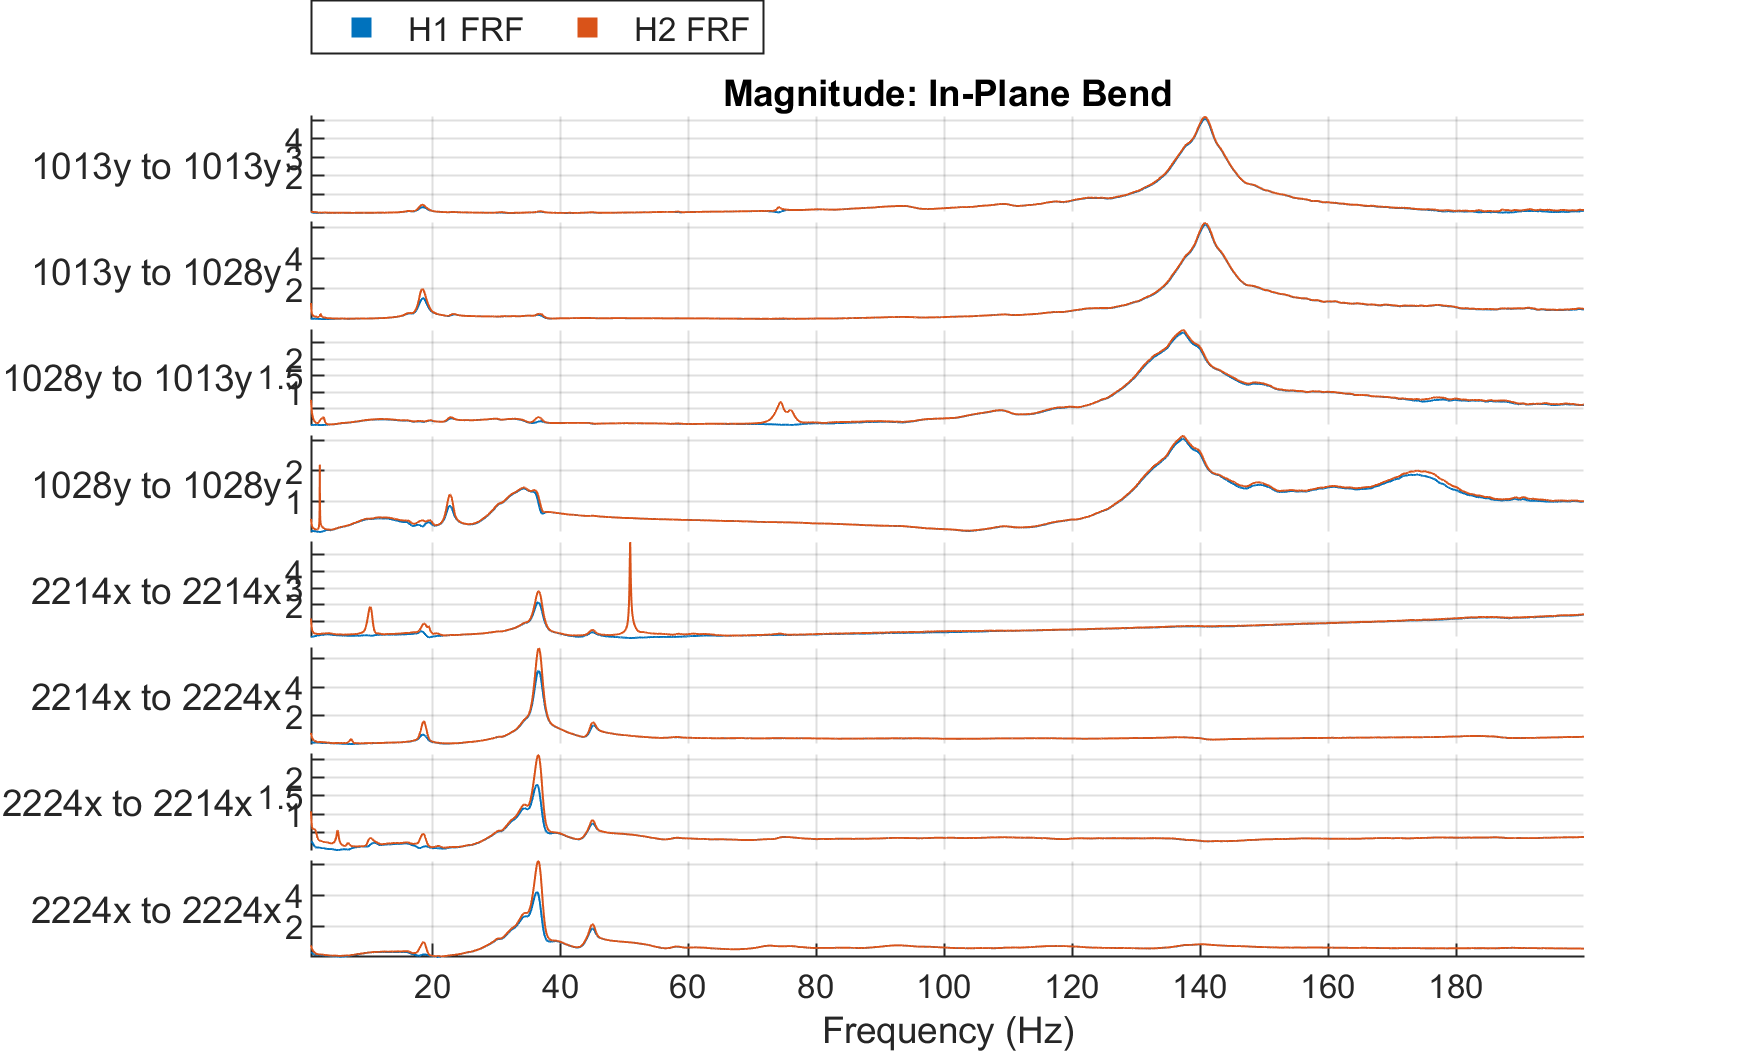
\includegraphics{figs/GVT/mag_In-Plane Bend.png}    
    \label{fig:mag_inPlaneBend}
\end{figure}
\begin{figure}[H]
    \centering
    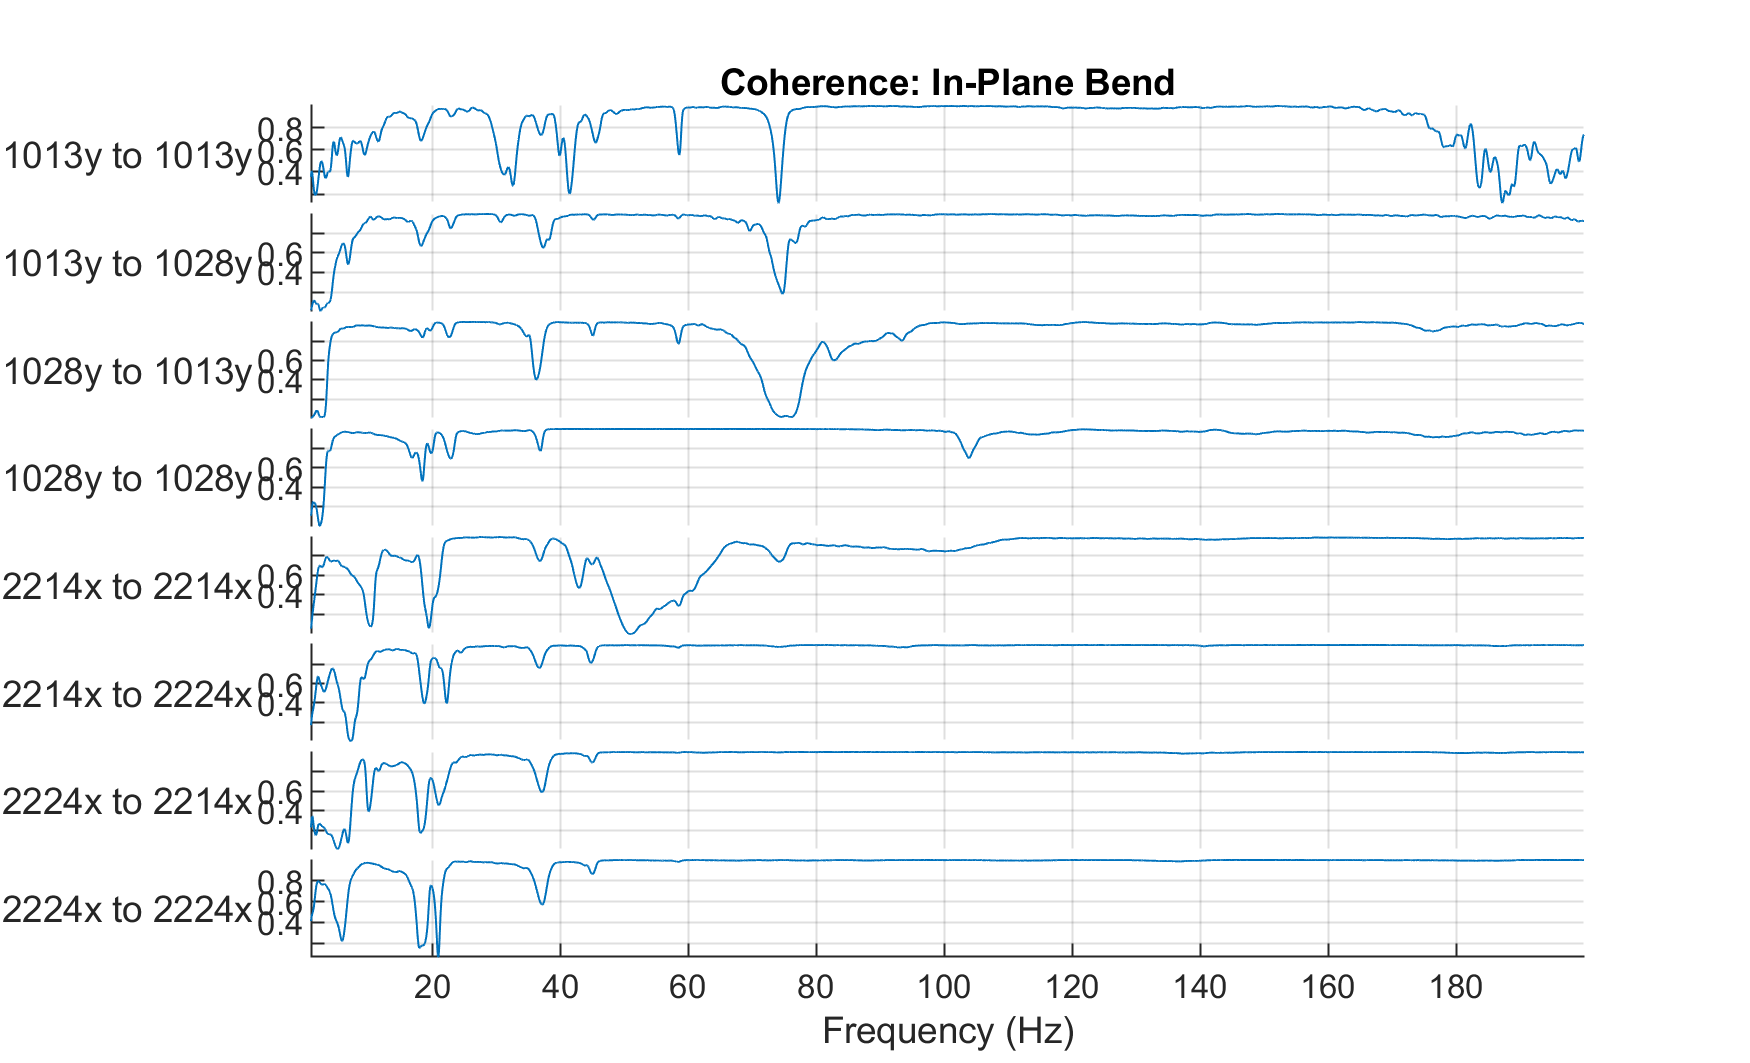
\includegraphics{figs/GVT/coh_In-Plane Bend.png}
    \label{fig:coh_inPlaneBend}
\end{figure}

\begin{figure}[H]
    \centering
    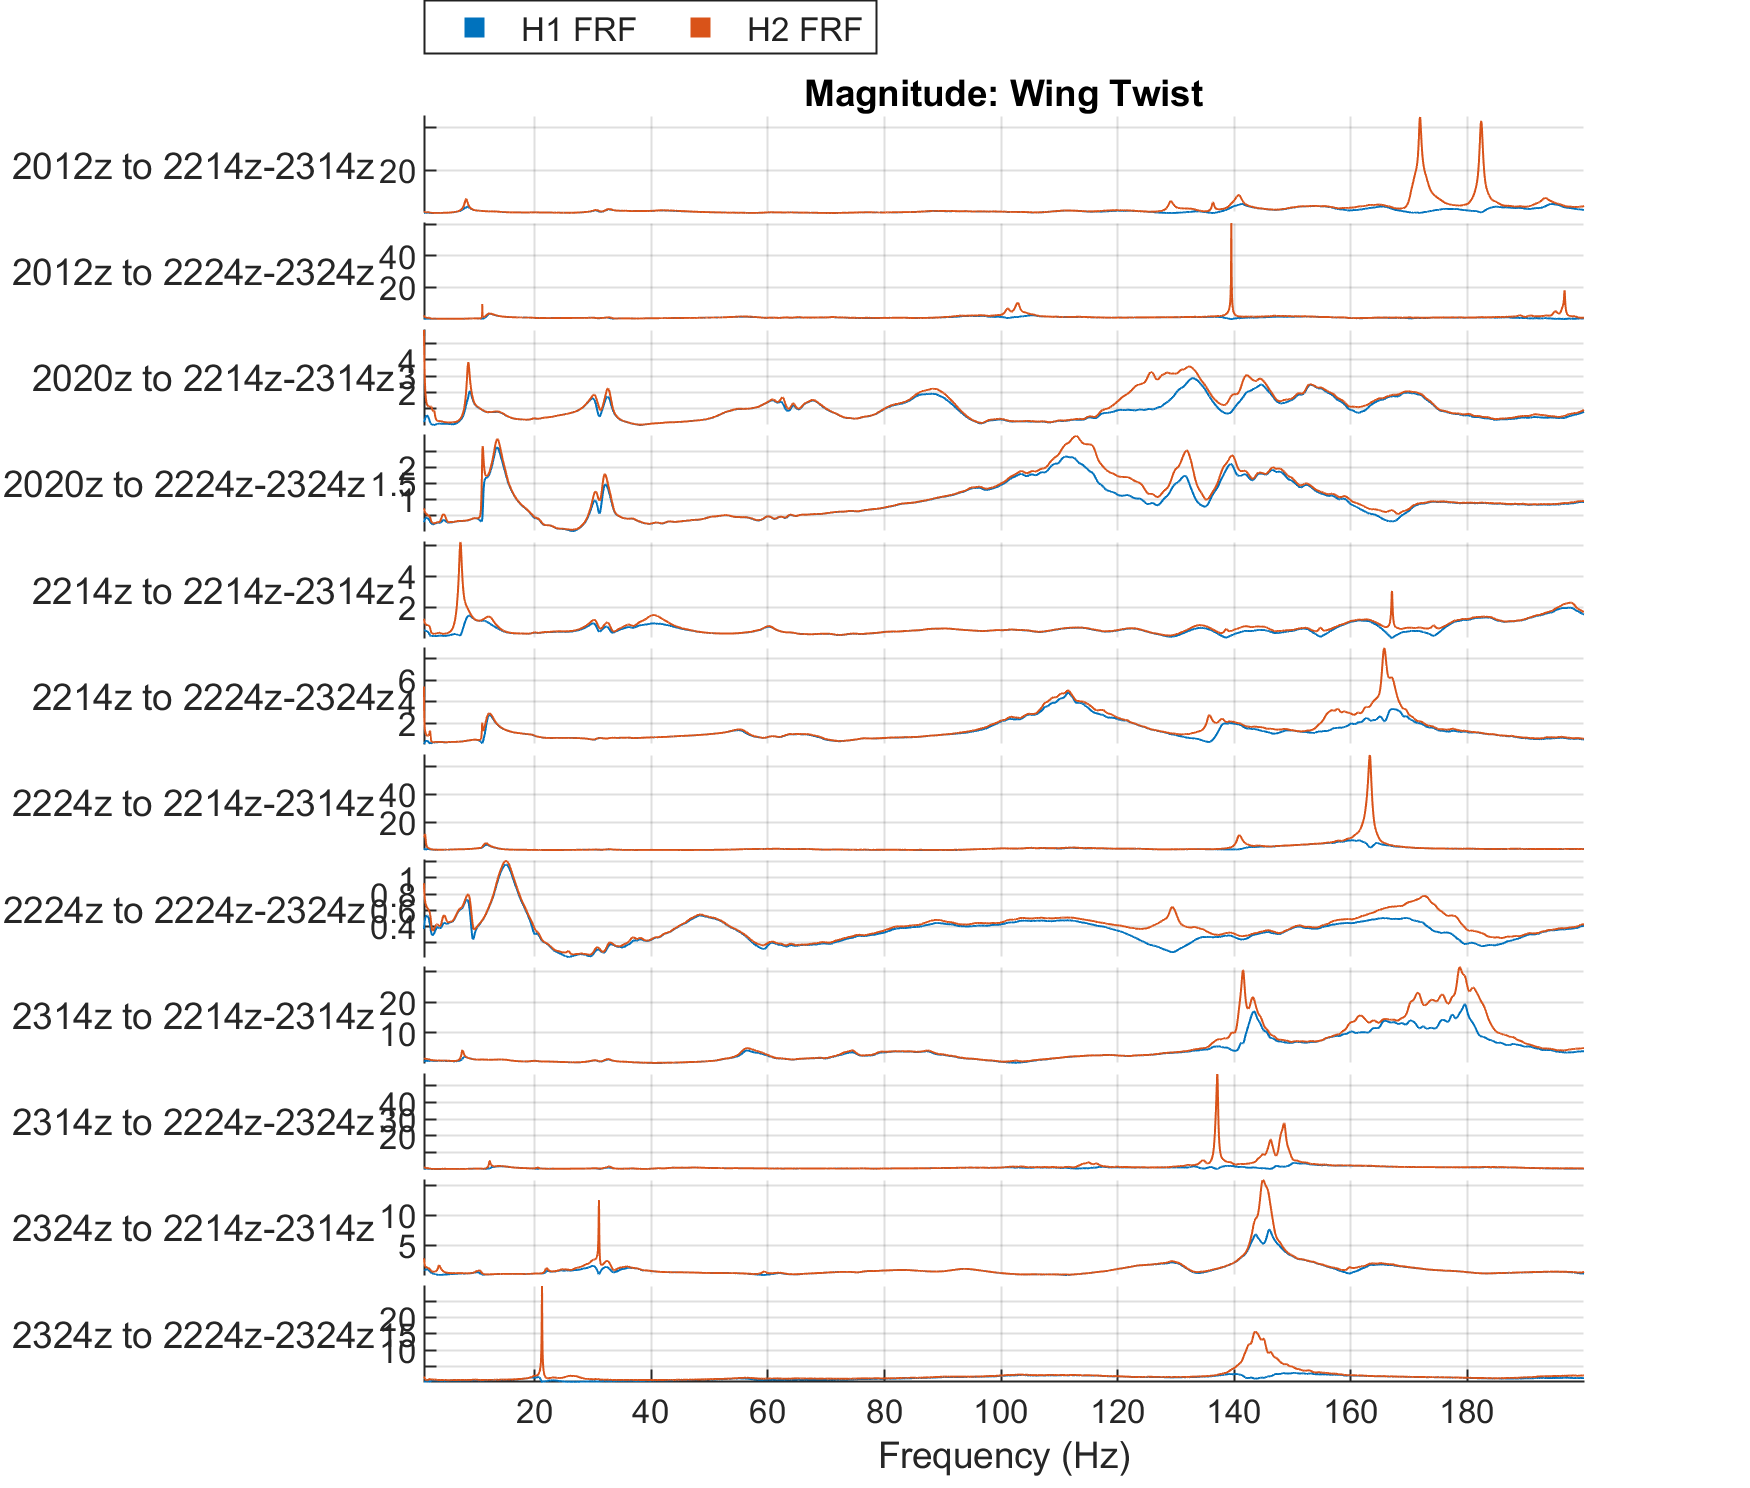
\includegraphics{figs/GVT/mag_Wing Twist.png}
    \label{fig:mag_wingTwist}
\end{figure}
\begin{figure}[H]
    \centering
    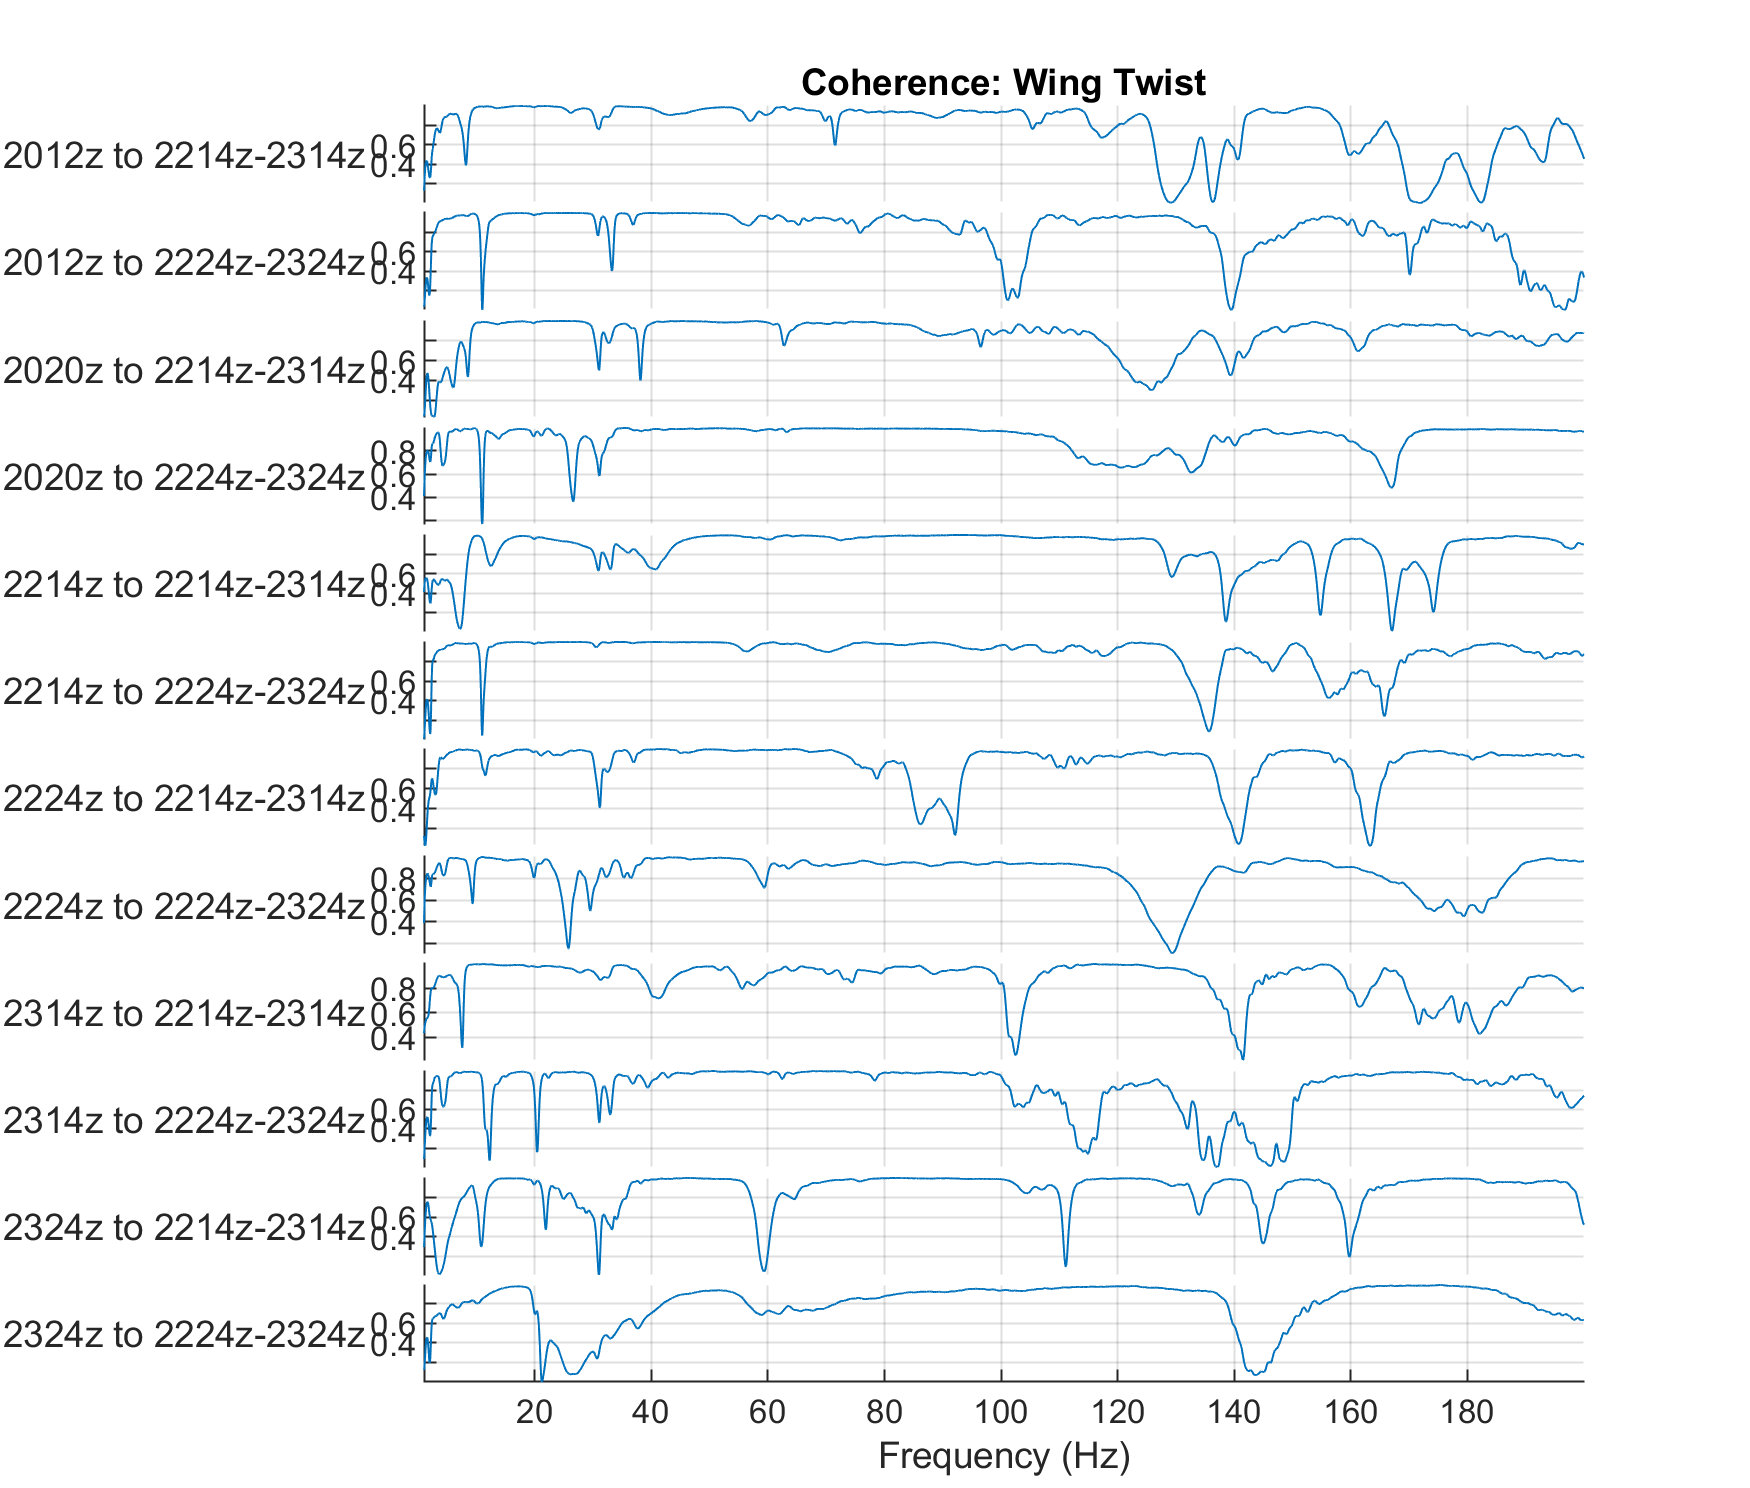
\includegraphics{figs/GVT/coh_Wing Twist.png} 
    \label{fig:coh_wingTwist}
\end{figure}

%%%%%%%%%%%%%%%%%%%%%%%%%%%%%%%%%%%%%%%%%%%%%%%%%%%%%%%%%%%%%%%%%%%
\section{Wind Tunnel Testing and Mathematical Models} %%%%%%%%%%%%%
%%%%%%%%%%%%%%%%%%%%%%%%%%%%%%%%%%%%%%%%%%%%%%%%%%%%%%%%%%%%%%%%%%%

Unless otherwise noted, mathematical models demonstrated in this section have $n_s=2$, $N_\text{lag}=0$, and physically bounded tuning variables as defined in Table \ref{tab:optBounds}

\begin{landscape}

\begin{figure}[H]
    \centering
    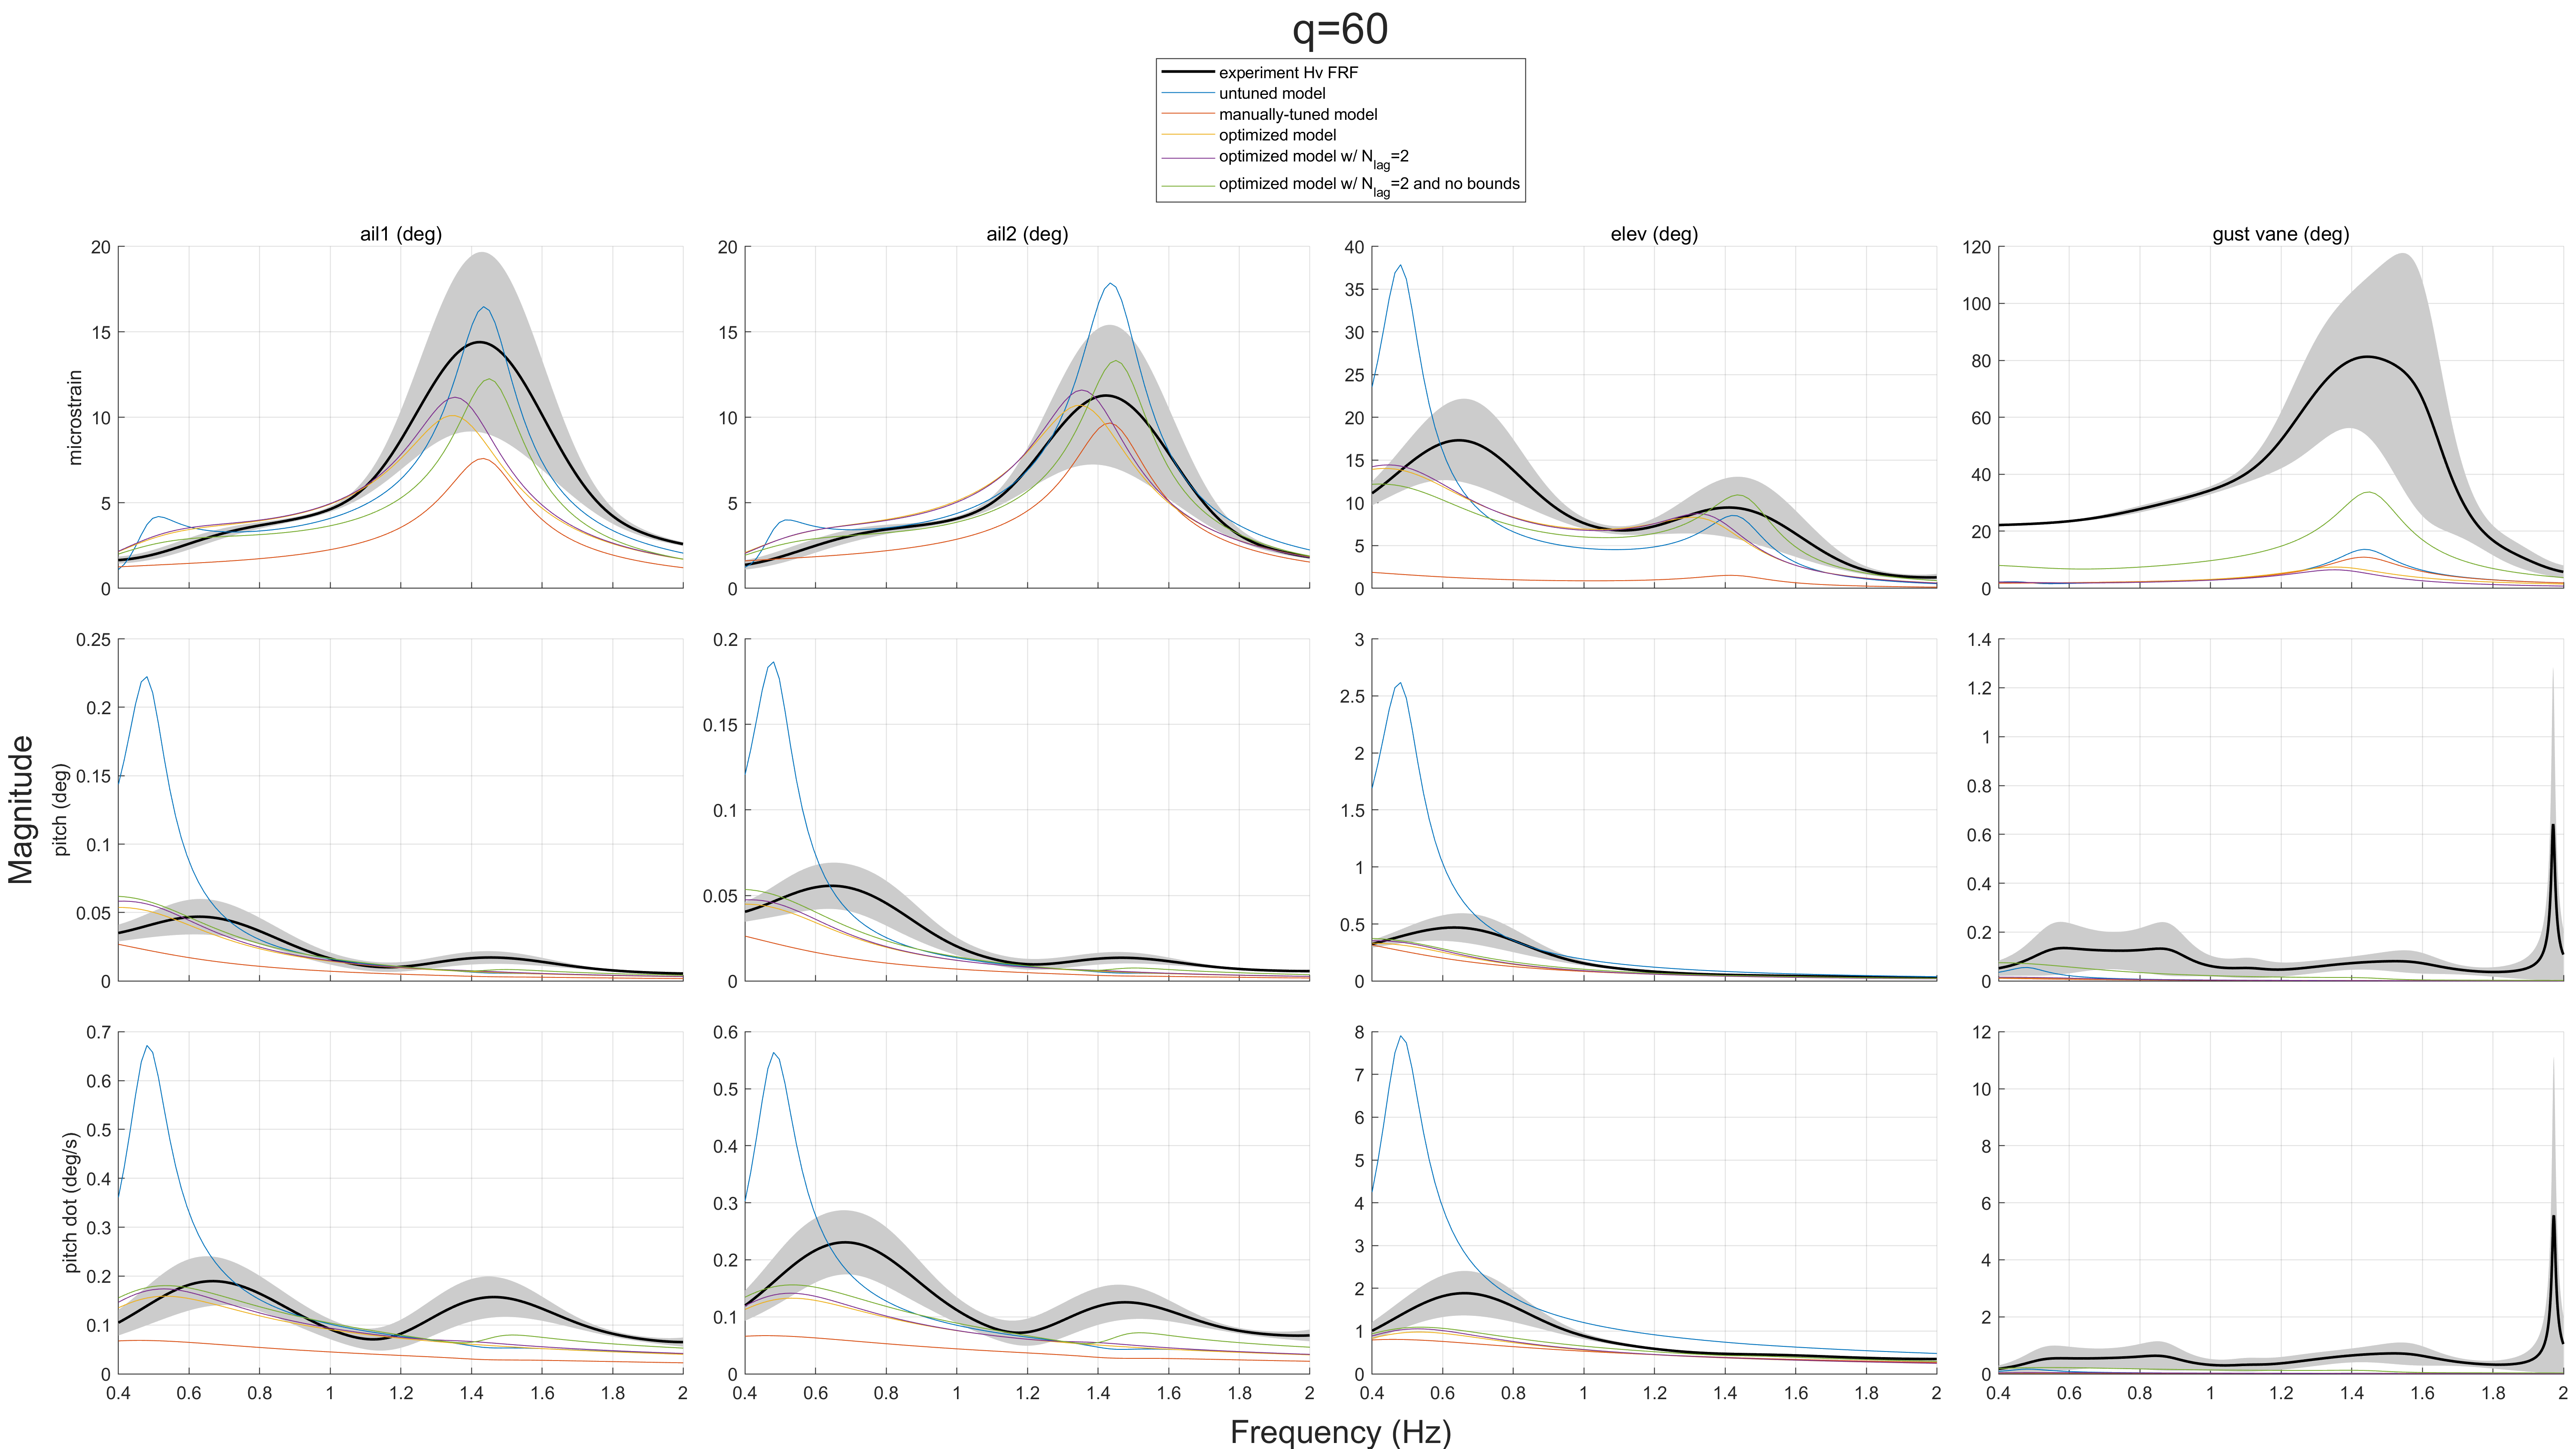
\includegraphics[width=9in]{figs/optFRFplot/FRFCOMPARE_MODEL_COMPARISON_q60.png} 
    \label{fig:optFRFplot_q60}
\end{figure}

\begin{figure}[H]
    \centering
    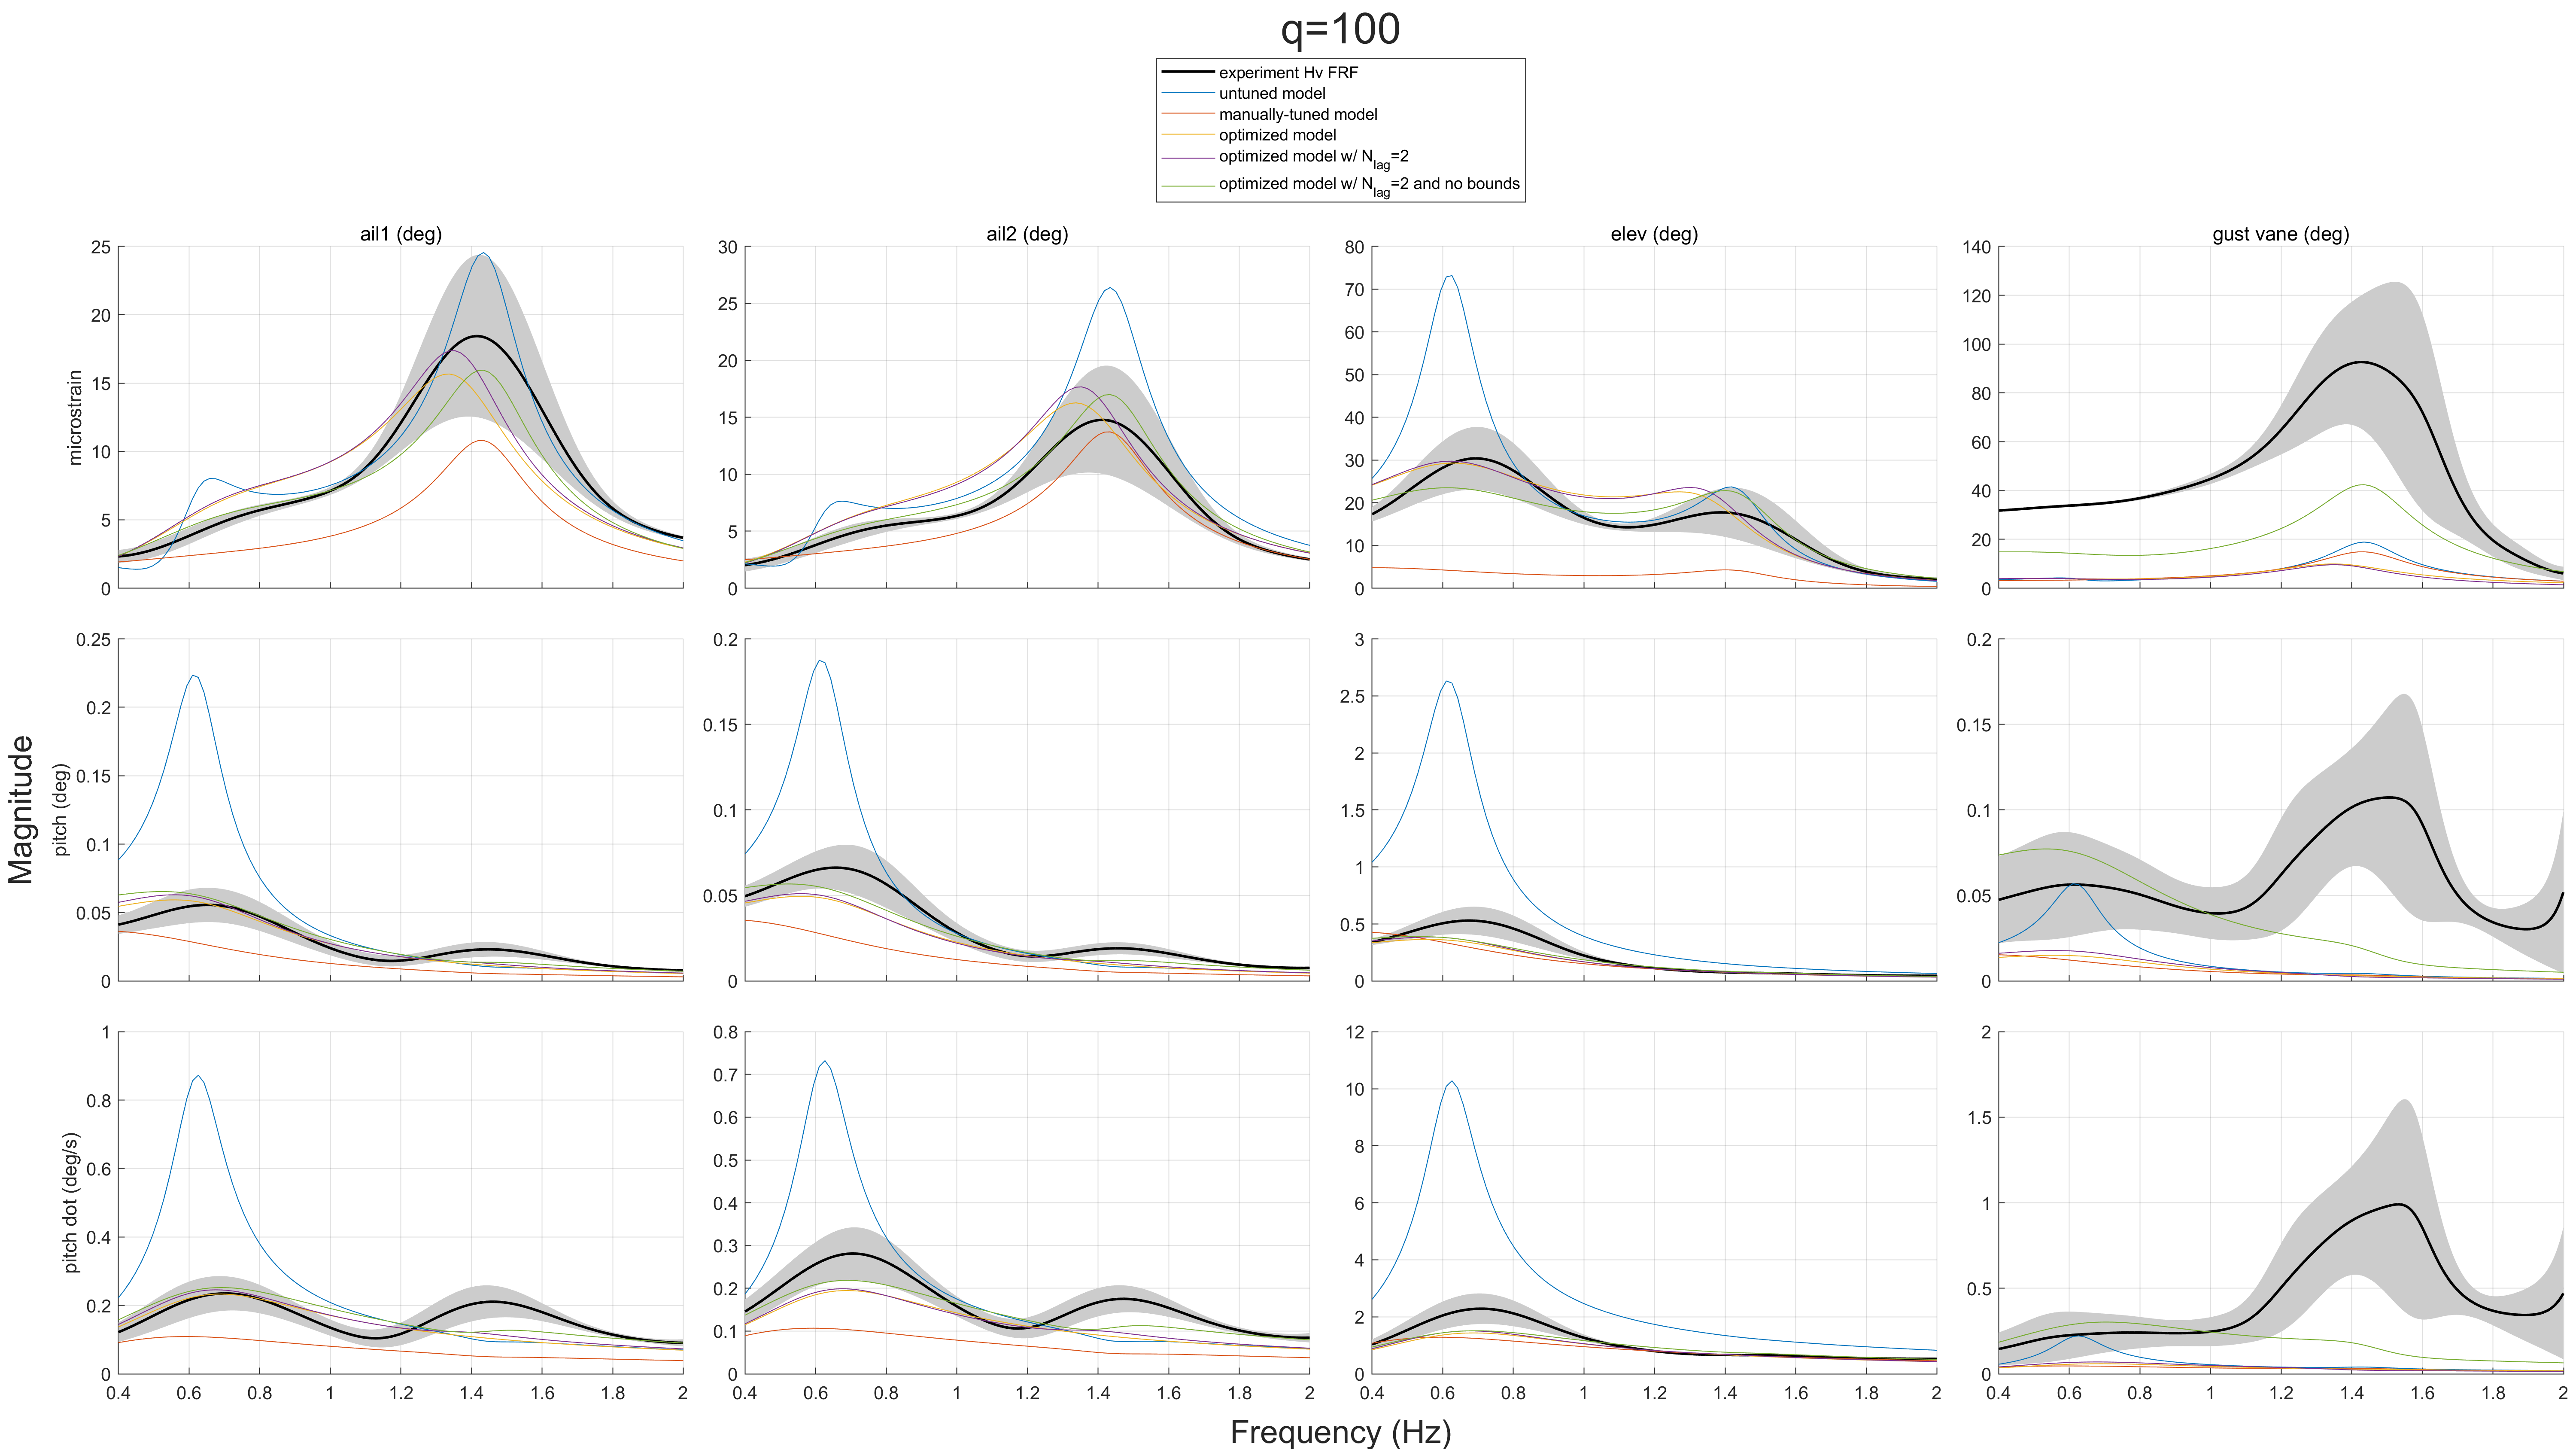
\includegraphics[width=9in]{figs/optFRFplot/FRFCOMPARE_MODEL_COMPARISON_q100.png} 
    \label{fig:optFRFplot_q100}
\end{figure}

\begin{figure}[H]
    \centering
    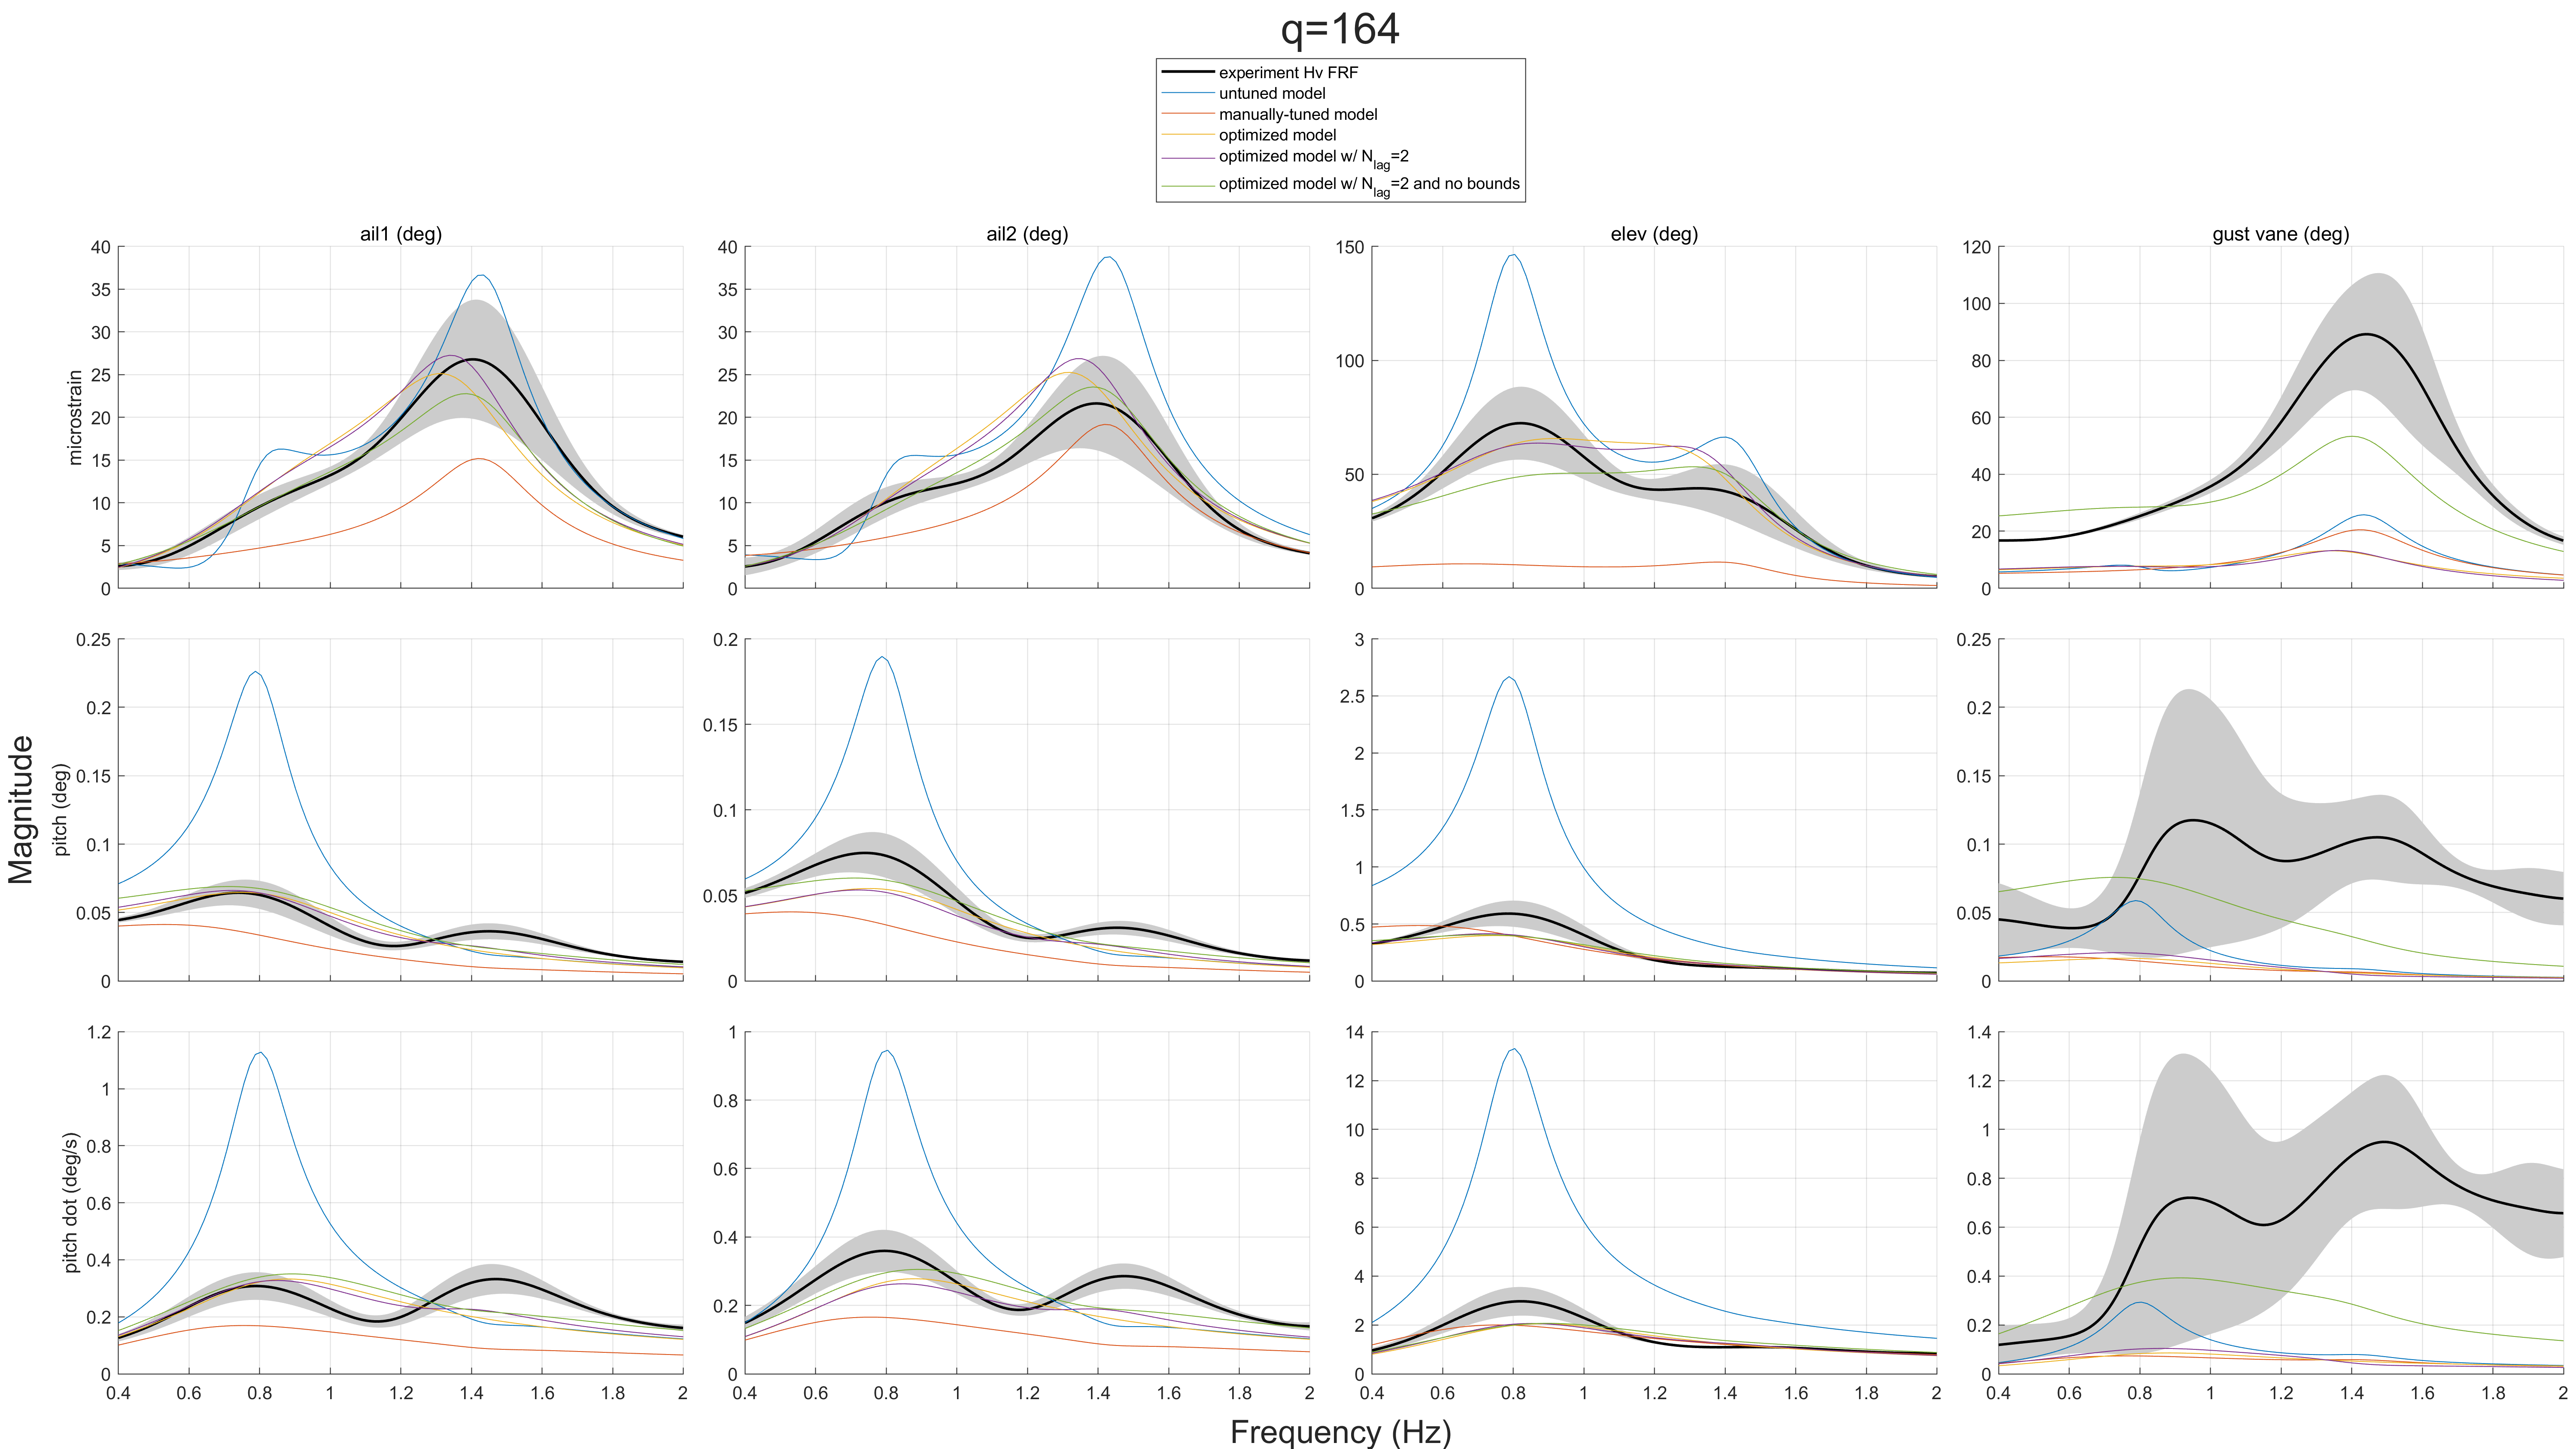
\includegraphics[width=9in]{figs/optFRFplot/FRFCOMPARE_MODEL_COMPARISON_q164.png} 
    \label{fig:optFRFplot_q164}
\end{figure}

\begin{figure}[H]
    \centering
    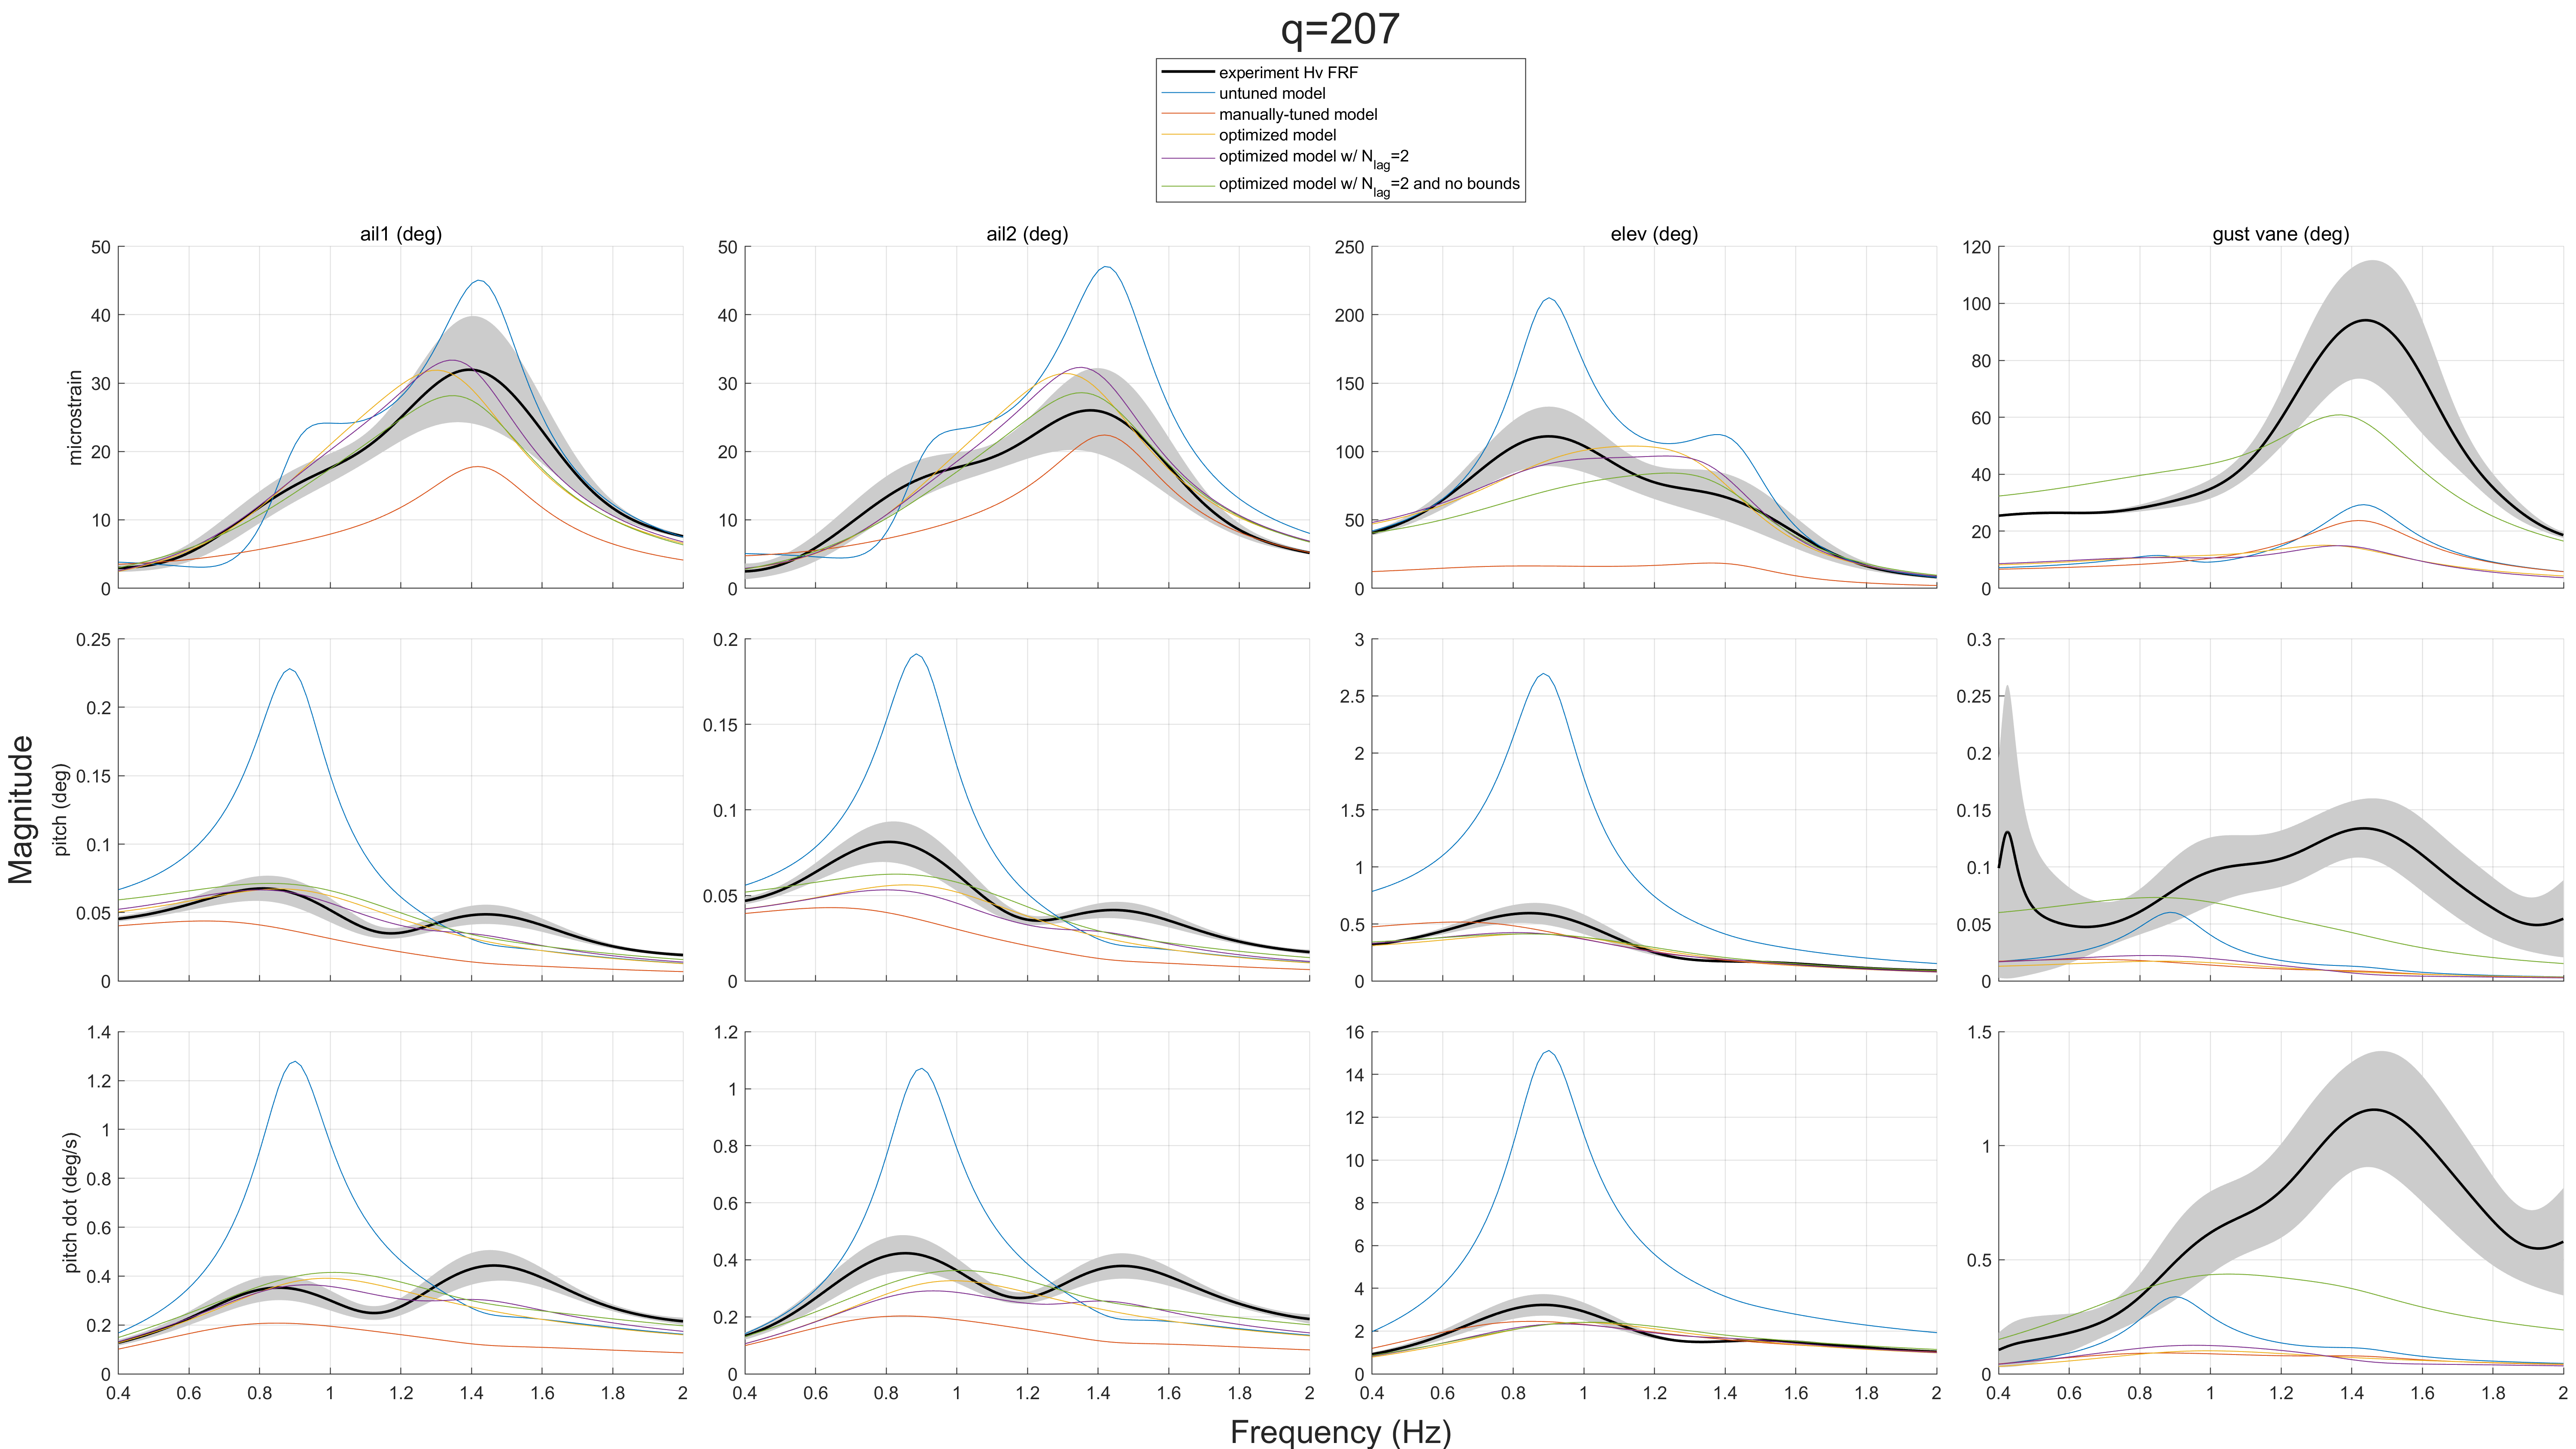
\includegraphics[width=9in]{figs/optFRFplot/FRFCOMPARE_MODEL_COMPARISON_q207.png} 
    \label{fig:optFRFplot_q207}
\end{figure}

\begin{figure}[H]
    \centering
    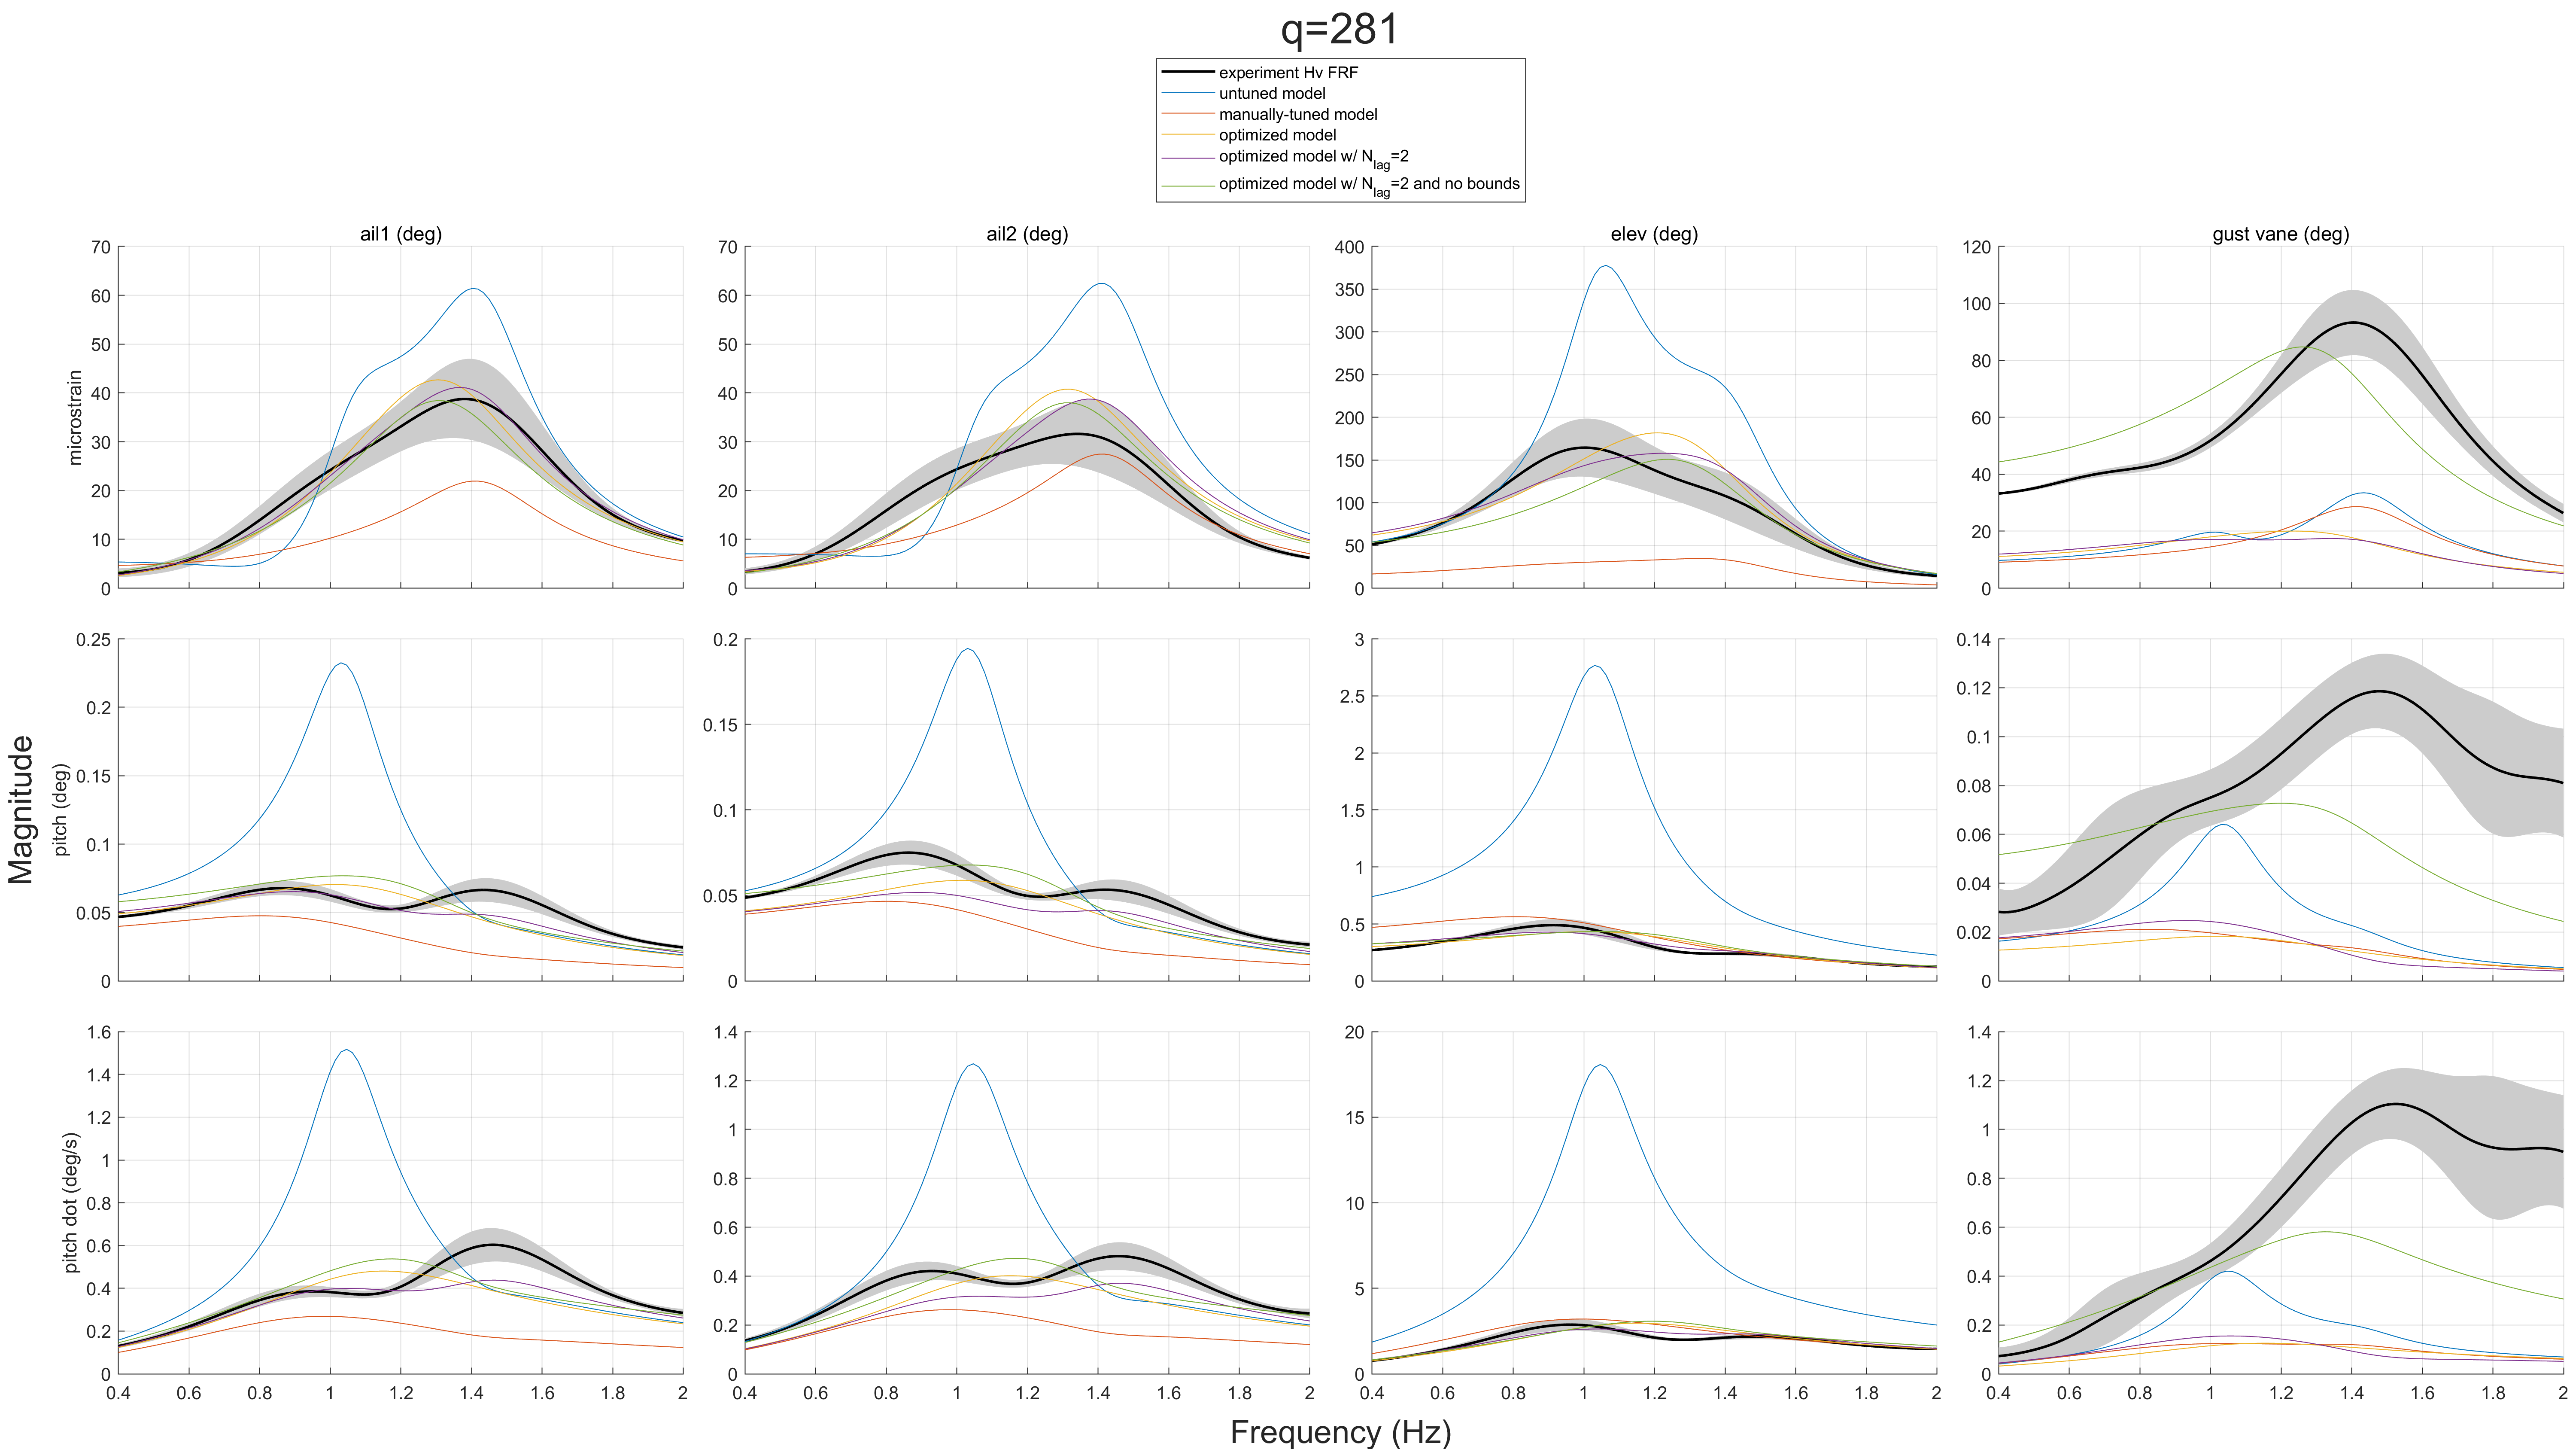
\includegraphics[width=9in]{figs/optFRFplot/FRFCOMPARE_MODEL_COMPARISON_q281.png} 
    \label{fig:optFRFplot_q281}
\end{figure}

\begin{figure}[H]
    \centering
    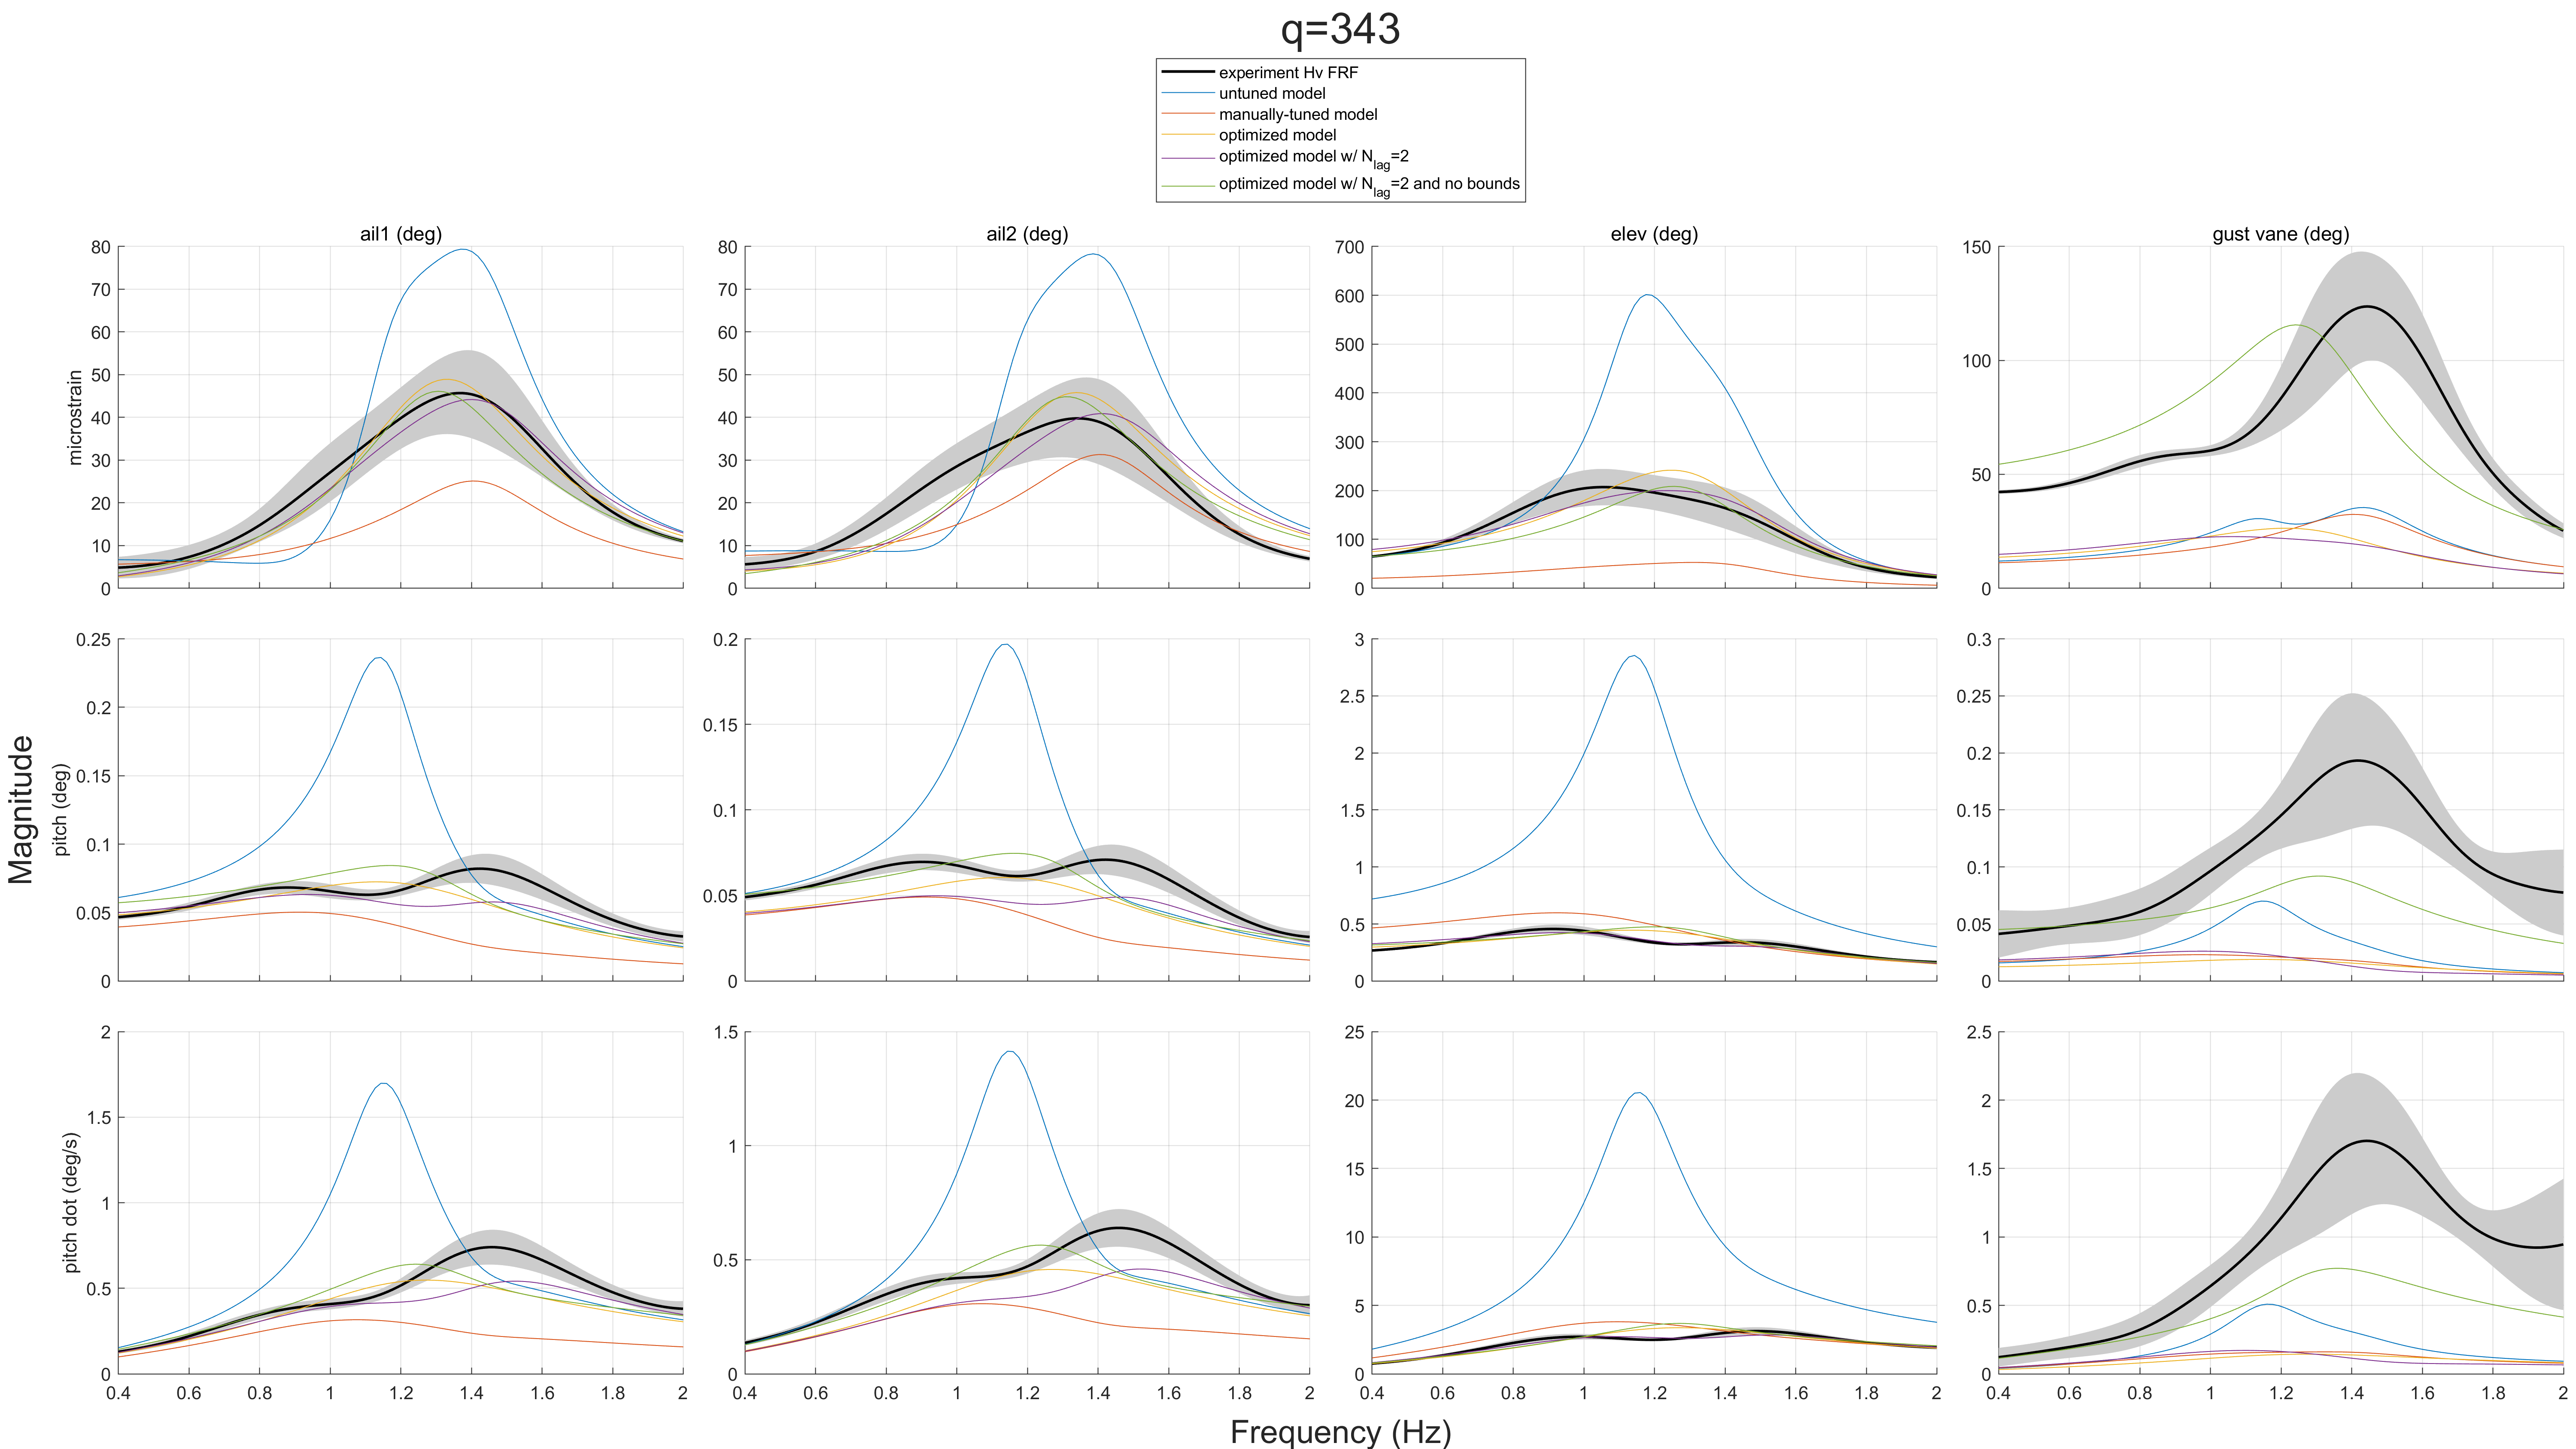
\includegraphics[width=9in]{figs/optFRFplot/FRFCOMPARE_MODEL_COMPARISON_q343.png} 
    \label{fig:optFRFplot_q343}
\end{figure}


\end{landscape}